% !TeX encoding = UTF-8
% !TeX program  = pdflatex
%
% relatorio_tcc.tex
% Relatório Final — TCC de MBA
% Escola Superior de Agricultura "Luiz de Queiroz" — ESALQ/USP
% Compilar: pdflatex → bibtex → pdflatex → pdflatex
% Ou: Upload em Overleaf (recomendado)
%
\documentclass[12pt, a4paper, oneside]{article}

% ── Encoding e língua ─────────────────────────────────────────────────────────
\usepackage[utf8]{inputenc}
\usepackage[T1]{fontenc}
\usepackage[brazil]{babel}
\usepackage{lmodern}

% ── Layout ────────────────────────────────────────────────────────────────────
\usepackage[top=3cm, bottom=2cm, left=3cm, right=2cm]{geometry}
\usepackage{setspace}
\onehalfspacing
\usepackage{indentfirst}
\setlength{\parindent}{1.25cm}

% ── Matemática ────────────────────────────────────────────────────────────────
\usepackage{amsmath, amssymb, amsthm}

% ── Figuras e tabelas ─────────────────────────────────────────────────────────
\usepackage{graphicx}
\usepackage{float}
\usepackage{booktabs}
\usepackage{longtable}
\usepackage{multirow}
\usepackage{tabularx}
\usepackage{caption}
\usepackage{subcaption}
\usepackage{xcolor}
\usepackage{array}

% ── Referências ───────────────────────────────────────────────────────────────
\usepackage[alf, abnt-etal-list=5]{abntex2cite}

% Unicode minus sign (U+2212) → LaTeX math minus
\DeclareUnicodeCharacter{2212}{$-$}

% Compatibility: abntex2cite with article class
\makeatletter
\providecommand{\abntnextkey}{}
\makeatother

% ── Hiperlinks ───────────────────────────────────────────────────────────────
\usepackage[colorlinks=true, linkcolor=black, citecolor=black, urlcolor=blue]{hyperref}

% ── Caminho das figuras ───────────────────────────────────────────────────────
\graphicspath{{outputs/figures/}}

\begin{document}

% ══════════════════════════════════════════════════════════════════════════════
%  CAPA
% ══════════════════════════════════════════════════════════════════════════════
\begin{titlepage}
\centering
\vspace*{1cm}

\IfFileExists{logo_esalq.pdf}{\includegraphics[width=4cm]{logo_esalq}}{%
  \framebox[4cm]{\rule{0pt}{1.5cm}\textit{Logo ESALQ}}%
}

\vspace{1.5cm}
{\Large \textbf{ESCOLA SUPERIOR DE AGRICULTURA ``LUIZ DE QUEIROZ''\\
UNIVERSIDADE DE SÃO PAULO}}

\vspace{1cm}
{\large MBA em Data Science e Analytics}

\vspace{3cm}

{\LARGE \textbf{RACISMO ESTRUTURAL NO MERCADO DE TRABALHO BRASILEIRO:
UMA ABORDAGEM MULTINÍVEL, DE MACHINE LEARNING, REDES SOCIAIS
E PESQUISA OPERACIONAL COM DADOS DA PNAD CONTÍNUA (2016--2025)}}

\vspace{3cm}

{\large \textbf{Ricardo Calheiros}}

\vfill

{\large Piracicaba, 2026}
\end{titlepage}

\newpage

% ══════════════════════════════════════════════════════════════════════════════
%  RESUMO
% ══════════════════════════════════════════════════════════════════════════════
\begin{abstract}
\noindent
Este trabalho investiga o \textit{gap} salarial racial e as barreiras
estruturais à progressão de carreira de profissionais negros no Brasil,
combinando econometria multinível, \textit{machine learning} e análise de
redes sociais sobre a série histórica completa da Pesquisa Nacional por
Amostra de Domicílios Contínua (PNAD Contínua) de 2016 a 2025, com
15,9~milhões de observações brutas.

Um modelo de regressão multinível de três níveis (indivíduo, UPA e Unidade
da Federação) estima que profissionais negros recebem, em média,
19.1\% a menos que brancos comparáveis em escolaridade, sexo e faixa etária.
Desse diferencial bruto, 52.5\% é mediado pelo contexto de moradia
(\textit{networking} local, Nível~2), reduzindo o \textit{gap} líquido
--- atribuível à discriminação direta --- a 9.6\%.

A análise de agrupamento (\textit{K-Means}, $k=3$) segrega a força de trabalho
em três tipologias socioeconomicamente distintas e racialmente homogêneas,
com trabalhadores negros concentrados nos grupos de menor rendimento e as
mulheres negras formando um cluster de dupla desvantagem (raça \textit{e}
gênero).

Modelos de \textit{Random Forest} e XGBoost com valores SHAP confirmam que
a renda média da UPA é o preditor mais importante do rendimento individual
($|\text{SHAP}| = 0.269$), seguida de gênero e escolaridade superior,
com a variável racial ocupando o 11$^\circ$ lugar mesmo após
controlar por todos os demais fatores.

A análise de redes sociais revela que grupos negros possuem
\textit{betweenness centrality} nula em todos os níveis educacionais,
enquanto grupos brancos de escolaridade fundamental e pós-graduação
funcionam como \textit{brokers} da rede de co-residência --- evidência
de que a conversão de capital humano em renda depende de capital social
estruturalmente negado a trabalhadores negros.

A pesquisa operacional traduz esses achados em recomendações concretas:
o método TOPSIS ranqueia seis políticas públicas avaliadas em cinco
critérios simultâneos, apontando as Cotas Ocupacionais CBO~1--4 como
política dominante (CC~$=0,8344$), seguida da
Equidade Educacional (CC~$=0,5879$).
A programação linear indica que uma alocação ótima de R\$5~bilhões,
priorizando os três canais de maior efetividade, reduziria o
\textit{gap} salarial racial em 25,1\%.

\bigskip
\noindent\textbf{Palavras-chave:} gap salarial racial; discriminação estrutural; modelos
hierárquicos lineares; SHAP values; análise de redes sociais; pesquisa
operacional; TOPSIS; programação linear; políticas públicas; PNAD Contínua.
\end{abstract}

\newpage

% ══════════════════════════════════════════════════════════════════════════════
%  ABSTRACT (English)
% ══════════════════════════════════════════════════════════════════════════════
\renewcommand{\abstractname}{Abstract}
\begin{abstract}
\noindent
This study investigates the racial wage gap and structural barriers to career
progression for Black professionals in Brazil using a multilevel, machine
learning, and social network analysis framework applied to the full historical
series of Brazil's Continuous National Household Sample Survey (PNAD Contínua)
from 2016 to 2025 (15.9~million raw observations).

A three-level hierarchical linear model (individual, census tract, and state)
estimates that Black workers earn 19.1\% less than comparable White
workers after controlling for education, sex, and age experience.
Of this gross differential, 52.5\% is mediated by residential context
(local networking, Level~2), leaving a residual \textit{net gap} of
9.6\% attributable to direct labour market discrimination.

K-Means clustering ($k=3$) reveals three racially homogeneous
socioeconomic typologies, with Black workers concentrated in lower-income
segments and Black women forming a dual-disadvantage cluster at the
intersection of race and gender.

Random Forest and XGBoost models with SHAP values confirm that neighbourhood
income is the most important predictor of individual earnings
($|\text{SHAP}|=0.269$), while race ranks
11$^\text{th}$ even after all controls.

Social network analysis shows that Black groups have zero betweenness
centrality regardless of education level, whereas White groups serve as
brokers in the co-residence network, suggesting that the conversion of
human capital into earnings depends on social capital that is structurally
denied to Black workers.

An operations research module translates these findings into policy
recommendations. A TOPSIS multicriteria ranking of six public policies
across five criteria identifies occupational quotas for CBO groups~1--4
as the dominant policy (CC~$=0,8344$), followed by
educational equity (CC~$=0,5879$). Linear programming
shows that an optimal R\$5-billion allocation would reduce the racial
wage gap by 25,1\%.

\bigskip
\noindent\textbf{Keywords:} racial wage gap; structural discrimination;
hierarchical linear models; SHAP values; social network analysis;
operations research; TOPSIS; linear programming; public policy; PNAD Contínua.
\end{abstract}

\newpage
\tableofcontents
\newpage

% ══════════════════════════════════════════════════════════════════════════════
%  1. INTRODUÇÃO
% ══════════════════════════════════════════════════════════════════════════════
\section{Introdução}
\label{sec:intro}

\begin{quote}
\textbf{Este trabalho comprova que o racismo no mercado de trabalho brasileiro
não opera como um evento isolado de discriminação salarial --- opera como
um sistema de barreiras em camadas que começa antes do primeiro salário,
persiste ao longo de toda a trajetória profissional e se perpetua via
exclusão das redes que convertem educação em mobilidade.
Políticas baseadas apenas em aumento de escolaridade são, portanto,
necessárias, mas estruturalmente insuficientes.}
\end{quote}

O Brasil é um dos países com maior desigualdade racial de renda no mundo.
Segundo a PNAD Contínua, a razão entre o rendimento médio de trabalhadores
brancos e negros permanece acima de 1{:}1,5 ao longo de toda a série
histórica disponível, persistindo mesmo quando se controlam escolaridade,
experiência e setor de atividade~\cite{ibge_pnad_2023}.
A desigualdade racial no mercado de trabalho brasileiro é, portanto,
não apenas uma herança colonial, mas um fenômeno reproduzido ativamente
por mecanismos que a abordagem tradicional de diferenças de capital humano
não é capaz de capturar~\cite{hasenbalg1979}.

Esse hiato convive com um quadro macroestrutural recente de \textbf{avanço social
com desigualdade persistente}. De um lado, a qualidade de vida avançou: entre as
edições 2008 e 2018 da Pesquisa de Orçamentos Familiares (POF), o Índice de Perda
de Qualidade de Vida recuou cerca de 30\%~\cite{ibge_pof_2019}. A melhora, porém,
foi proporcional entre os grupos e \emph{não} fechou o hiato racial nem o
territorial: famílias chefiadas por pessoas pretas ou pardas mantêm índice de
0{,}183, contra 0{,}122 das brancas, e o Nordeste (0{,}207) e o Norte
(0{,}223) seguem muito acima do Sul (0{,}114). De outro lado, no rendimento, a
desigualdade voltou a crescer: o Gini do rendimento domiciliar \emph{per capita}
subiu de 0{,}487 (2024) para 0{,}491 (2025), puxado pelo distanciamento do topo
--- a renda dos 10\% mais ricos cresceu 8{,}7\% no ano, contra 3{,}1\% dos 10\%
mais pobres~\cite{ibge_rendimentos_2025}. É precisamente esse padrão --- progresso
agregado que não dissolve a barreira racial --- que este trabalho disseca no
mercado de trabalho.

A literatura empírica contemporânea identifica três canais principais de
reprodução dessa desigualdade: (i)~discriminação direta, isto é, diferenças
de tratamento em processos de seleção e promoção com características
individuais observadas~\cite{pager2007}; (ii)~segregação residencial e
seus efeitos sobre o capital social disponível ao trabalhador
--- o contexto do bairro define a qualidade das redes de indicação
profissional~\cite{wilson1987, sampson1997}; e (iii)~subvalorização
sistêmica do capital humano negro, pela qual um dado nível de escolaridade
gera retornos financeiros menores para trabalhadores negros do que para
brancos~\cite{hasenbalg1979, pager2007}.

Este trabalho avança sobre a literatura nacional ao integrar três
metodologias complementares --- econometria multinível, \textit{machine learning}
interpretável e análise de redes sociais --- sobre a maior base de dados
longitudinal disponível no Brasil para este tema, a PNAD Contínua em sua
série completa de 2016 a 2025.

\subsection{Hipóteses}
\label{subsec:hipoteses}

\begin{enumerate}
  \item[\textbf{H1}] \textbf{Gap racial bruto e líquido:}
    Profissionais negros apresentam rendimento inferior ao de brancos
    comparáveis após controlar por escolaridade, experiência potencial
    e gênero --- e esse diferencial persiste após a adição de controles
    contextuais de nível de bairro e de estado.

  \item[\textbf{H2}] \textbf{Mediação pelo networking local:}
    Uma fração significativa do \textit{gap} racial bruto é explicada
    pelo contexto socioeconômico do local de moradia (composição racial da
    UPA, desemprego local, nível educacional médio do entorno) ---
    capturando os efeitos indiretos da segregação residencial sobre a renda.

  \item[\textbf{H3}] \textbf{Tipologias de vulnerabilidade alinhadas com raça:}
    Métodos de agrupamento não-supervisionados identificam clusters
    socioeconômicos que se sobrepõem a fronteiras raciais, com trabalhadores
    negros concentrados nos segmentos de maior vulnerabilidade.

  \item[\textbf{H4}] \textbf{Importância residual da raça nos modelos preditivos:}
    Mesmo após controlar por educação, experiência, gênero e contexto de
    moradia, a variável racial mantém relevância preditiva independente,
    conforme medida pelos valores SHAP dos modelos de \textit{gradient boosting}.

  \item[\textbf{H5}] \textbf{Isolamento estrutural na rede de co-residência:}
    Grupos negros ocupam posições periféricas na rede demográfica de
    co-residência, com menor capacidade de corretagem (\textit{brokerage})
    entre grupos do que seus pares brancos de mesma escolaridade, o que
    limita a conversão do capital humano em rendimento.
\end{enumerate}

% ══════════════════════════════════════════════════════════════════════════════
%  2. REVISÃO DE LITERATURA
% ══════════════════════════════════════════════════════════════════════════════
\section{Revisão de Literatura}
\label{sec:revisao}

\subsection{Desigualdade racial no mercado de trabalho brasileiro}

\citeonline{hasenbalg1979} demonstrou pioneiramente que a desigualdade racial
no Brasil não decorre apenas de diferenças históricas de acesso à educação,
mas de mecanismos ativos de discriminação no mercado de trabalho que
convertem desvantagens sociais em desvantagens econômicas de forma cumulativa.
Trabalhos posteriores~\cite{henriques2001, soares2009} confirmaram a
persistência dessas diferenças mesmo após controlar por escolaridade,
reforçando a hipótese de discriminação estrutural.

\subsection{Efeitos de vizinhança e segregação residencial}

\citeonline{wilson1987} propôs a hipótese da \textit{concentrated disadvantage}:
a concentração de pobreza em bairros racialmente segregados amplifica
desvantagens individuais por meio da redução de redes de contato com
o mercado de trabalho formal, degradação de serviços públicos e aumento
da violência. \citeonline{sampson1997} forneceu evidência empírica para essa
hipótese em contexto norte-americano, e estudos brasileiros encontraram
padrões similares para as regiões metropolitanas~\cite{marques2010}.

A abordagem de \textit{networking} local, operacionalizada neste trabalho
pelo segundo nível do modelo hierárquico (UPA), testa se o contexto
socioeconômico do bairro exerce efeito independente sobre o rendimento
após controlar por características individuais --- o chamado
\textit{duplo disadvantage} de ser negro \textit{e} morar em bairros negros.

\subsection{Modelos lineares hierárquicos para dados aninhados}

\citeonline{raudenbush2002} sistematizaram a fundamentação estatística dos
modelos lineares hierárquicos (HLM), tornando-os o padrão metodológico para
análise de dados com estrutura aninhada (indivíduos dentro de bairros dentro
de estados). Esses modelos permitem decompor a variância do desfecho em
componentes de cada nível e estimar os efeitos contextuais
controlando simultaneamente pelos efeitos individuais.

\subsection{Interpretabilidade em machine learning: SHAP values}

\citeonline{lundberg2017} propuseram os \textit{SHapley Additive exPlanations}
(SHAP), unificando importância de variáveis, efeitos parciais e explicações
individuais em uma única estrutura axiomática baseada na teoria dos jogos
cooperativos. Para dados socioeconômicos, SHAP permite responder à pergunta:
``quanto e em que direção a raça de um indivíduo específico afeta a predição
de sua renda?'' --- uma contribuição metodológica que complementa e enriquece
a interpretação dos coeficientes do HLM.

\subsection{Análise de redes sociais e capital social}

\citeonline{granovetter1973} demonstrou que \textit{laços fracos} ---
conexões entre indivíduos de grupos sociais distintos --- são os principais
canais de transmissão de informações sobre oportunidades profissionais.
\citeonline{burt2004} formalizou o conceito de \textit{buraco estrutural}:
indivíduos que conectam grupos desconexos obtêm vantagens relacionais
(acesso antecipado a vagas, mentoria, promoções). Aplicado à questão racial,
a SNA permite investigar se trabalhadores negros ocupam as posições de rede
que possibilitam o aproveitamento dessas vantagens.

% ══════════════════════════════════════════════════════════════════════════════
%  3. DADOS E METODOLOGIA
% ══════════════════════════════════════════════════════════════════════════════
\section{Dados e Metodologia}
\label{sec:metodologia}

\subsection{Base de dados: PNAD Contínua (2016--2025)}

A PNAD Contínua é uma pesquisa amostral de domicílios conduzida
trimestralmente pelo IBGE, com cobertura nacional e metodologia de painel
rotativo. O microdado contém informações sobre características demográficas,
escolaridade, inserção no mercado de trabalho e rendimentos para todos os
moradores dos domicílios selecionados. Para este trabalho, foram processados
todos os 40~trimestres disponíveis de 2016T1 a 2025T4, totalizando
15.941.675~observações brutas, das quais 7.694.198 possuem renda positiva
declarada e completude nas variáveis do modelo.

A classificação racial segue o critério binário adotado pelos estudos
de desigualdade racial no Brasil: \textit{negro} = preto (código~2) +
pardo (código~4); \textit{branco} = branco (código~1), ambos da variável
V2010 (cor ou raça autodeclarada).

\subsection{Modelo Linear Hierárquico de Três Níveis}
\label{subsec:hlm}

O modelo parte da equação de Mincer estendida para o log-rendimento
mensal de trabalho, estruturada em três níveis:

\paragraph{Nível 1 --- Indivíduo ($i$) dentro da UPA ($j$) no Estado ($k$):}
\begin{equation}
  \ln(W)_{ijk} = \beta_{0jk}
    + \beta_1 \cdot \text{Negro}_{ijk}
    + \beta_2 \cdot \text{Sexo}_{ijk}
    + \beta_3 \cdot X_{ijk}
    + \beta_4 \cdot X^2_{ijk}
    + \sum_{e=1}^{4} \beta_{e+4} \cdot \text{Educ}_e
    + \varepsilon_{ijk}, \quad \varepsilon \sim \mathcal{N}(0,\sigma^2)
  \label{eq:nivel1}
\end{equation}

\paragraph{Nível 2 --- Localidade ($j$, proxy de bairro via UPA):}
\begin{equation}
  \beta_{0jk} = \gamma_{00k}
    + \gamma_{01} \cdot \overline{\%\text{Negro}}_{jk}
    + \gamma_{02} \cdot \overline{\text{Desemprego}}_{jk}
    + \gamma_{03} \cdot \overline{\text{Educ}}_{jk}
    + u_{0jk}, \quad u_{0j} \sim \mathcal{N}(0, \tau^2_u)
  \label{eq:nivel2}
\end{equation}

O coeficiente $\gamma_{01} < 0$ constitui evidência de \textit{duplo disadvantage}:
morar em bairros com maior concentração de negros reduz o rendimento
\textit{independentemente} da raça individual.

\paragraph{Nível 3 --- Estado ($k$, UF):}
\begin{equation}
  \gamma_{00k} = \delta_{000}
    + \delta_1 \cdot Z_k^{\%\text{negro}}
    + \delta_2 \cdot Z_k^{\text{desemprego}}
    + \delta_3 \cdot Z_k^{\text{educ}}
    + v_{00k}, \quad v_{00k} \sim \mathcal{N}(0, \tau^2_v)
  \label{eq:nivel3}
\end{equation}

Em um modelo de três níveis, o ICC completo é:
\begin{equation}
  \rho_{UF} = \frac{\tau^2_{UF}}{\tau^2_{UF} + \tau^2_{UPA} + \sigma^2}
  \label{eq:icc}
\end{equation}
onde $\tau^2_{UF}$ é a variância entre estados, $\tau^2_{UPA}$ a variância
entre UPAs e $\sigma^2$ a variância residual intraindividual.
Valores $\rho_{UF} > 0{,}05$ justificam a inclusão do nível~3 no modelo
\cite{raudenbush2002}.

Os efeitos de localidade (UPA) são modelados como \textit{interceptos fixos}
--- estratégia computacionalmente viável para 41.517 grupos e apropriada quando
o interesse reside em controlar heterogeneidade não observada de cada UPA,
sem necessidade de estimar a distribuição dos efeitos aleatórios de UPA.
Nessa especificação, $\tau^2_{UPA}$ não é estimado separadamente e a
fórmula do ICC de Nível~3 reduz-se a $\rho_{UF} = \tau^2_{UF} / (\tau^2_{UF} + \sigma^2)$,
reportada nas tabelas deste trabalho.
A estimação utiliza REML com método de Powell
para evitar colapso de variância na fronteira $\tau^2=0$.

\subsection{Clustering Socioeconômico (K-Means)}

O algoritmo \textit{MiniBatchKMeans} foi aplicado sobre as
$N=7.694.198$ observações da PEA completa com variáveis contextuais
disponíveis, usando 12~dimensões padronizadas: idade, três dummies de
escolaridade (ensino médio completo, superior completo, pós-graduação),
log-rendimento, raça, gênero, status de emprego e quatro variáveis de
contexto da UPA. O número ótimo de clusters foi determinado pelo
\textit{Silhouette Coefficient} \cite{rousseeuw1987} com validação
pelo índice de Davies-Bouldin \cite{davies_bouldin1979}.
Para $k=2$: $S=0,1736$, $DB=2,0140$;
para $k=3$: $S=0,1401$, $DB=2,2814$.
Ambos os critérios automáticos favorecem $k=2$; $k=3$ foi adotado por
interpretabilidade substantiva superior \cite{ketchen1996}, uma vez que
a solução binária reproduz trivialmente a clivagem racial sem discriminar
segmentos ocupacionais internos.

\subsection{Random Forest, XGBoost e SHAP Values}

Para predição do log-rendimento, foram ajustados dois modelos de ensemble:
(i)~\textit{Random Forest} \cite{breiman2001} com 200 árvores e profundidade
máxima 10; e (ii)~\textit{XGBoost} \cite{chen2016} com 300 iterações,
$\text{lr}=0{,}05$ e regularização $L_1/L_2$. Sobre o modelo XGBoost,
foi aplicado o \textit{TreeExplainer} da biblioteca SHAP
\cite{lundberg2017} sobre um subsample de 50.000 observações para
calcular os valores de Shapley de cada feature.

\subsection{Análise de Redes Sociais (SNA)}

A rede demográfica expandida foi construída com $N_{nós}=20$~nós,
representando as combinações de raça~$\times$~educação~$\times$~gênero
(2 raças $\times$ 5 níveis $\times$ 2 gêneros), e arestas ponderadas
pelo índice de Jaccard de co-presença em UPAs:
\begin{equation}
  w_{AB} = \frac{|\mathcal{U}_A \cap \mathcal{U}_B|}
                   {|\mathcal{U}_A \cup \mathcal{U}_B|}
  \label{eq:jaccard}
\end{equation}
onde $\mathcal{U}_A$ é o conjunto de UPAs com trabalhadores do grupo~$A$.
A expansão para 20~nós acrescenta a dimensão de gênero, aumentando a
robustez das métricas de centralidade e permitindo detectar posições de
\textit{brokerage} por subgrupo interseccional (raça~$\times$~gênero).
As métricas de rede incluem centralidade de grau, \textit{betweenness},
\textit{clustering coefficient} e \textit{constraint} de Burt~\cite{burt2004}.

\paragraph{Escopo macroestrutural da rede.}
Cabe uma delimitação conceitual: a PNAD Contínua não registra vínculos sociais
interpessoais, de modo que esta não é uma rede de \textit{indivíduos}, mas de
\textbf{grupos demográficos}. Os nós agregam estratos de raça, escolaridade e
gênero, e as arestas medem \textit{co-residência} na mesma UPA --- o substrato
territorial sobre o qual as redes interpessoais efetivamente se formam. Em
consequência, \textit{betweenness} e \textit{constraint} devem ser
interpretados como \textbf{posição estrutural de grupos} no espaço da
segregação residencial, e não como intermediação interpessoal medida. A SNA aqui
não substitui um estudo de laços egocêntricos; ela revela o \textit{andaime
macroestrutural} que condiciona, a montante, quem tem acesso a quais círculos
--- complementando, e não duplicando, as barreiras de acesso (GLMM) e de
remuneração (HLM).

% ══════════════════════════════════════════════════════════════════════════════
%  4. RESULTADOS
% ══════════════════════════════════════════════════════════════════════════════
\section{Resultados}
\label{sec:resultados}

As evidências deste capítulo estão organizadas em três camadas de exclusão
--- três barreiras que operam em sequência e se reforçam mutuamente.
O leitor não encontrará aqui um catálogo de modelos estatísticos:
encontrará a trajetória de um trabalhador negro no mercado de trabalho
brasileiro, documentada com rigor empírico em cada etapa.

\begin{table}[ht]
\centering
\caption{Mapa das três camadas de exclusão racial --- guia de leitura}
\label{tab:mapa_barreiras}
\begin{tabularx}{\textwidth}{|l|X|}
\hline
\textbf{Camada} & \textbf{Pergunta central e evidência} \\
\hline
\textbf{BARREIRA I} & Por que negros raramente chegam às ocupações de \\
\textbf{Acesso e Segregação} & prestígio? GLMM ($N=7.694.198$), HLM contextual e segregação \\
 & espacial mostram que a exclusão começa antes do salário. \\
\hline
\textbf{BARREIRA II} & Para os que superam a barreira de entrada --- qual é o \\
\textbf{Penalidade e Teto de Vidro} & custo de ser negro? Gap residual de -6.2\% após 23 controles, \\
 & crescendo nos quantis mais altos (KB-test $p<0{,}001$). \\
\hline
\textbf{BARREIRA III} & Por que educação, sozinha, não quebra o ciclo? \\
\textbf{Isolamento Estrutural} & Redes sociais com betweenness nulo para todos os grupos \\
 & negros: capital social transita exclusivamente por atores brancos. \\
\hline
\end{tabularx}
\end{table}

\medskip

Cada seção a seguir prova empiricamente uma dessas camadas.
Nenhum método isolado teria identificado o sistema como um todo.

\noindent\rule{\textwidth}{1pt}
\textbf{\large BARREIRA I --- ACESSO E SEGREGAÇÃO ESTRUTURAL}
\textit{Como a exclusão começa antes do primeiro salário}
\noindent\rule{\textwidth}{1pt}

\subsection{Modelos Hierárquicos Lineares --- Mediação Contextual do Gap}
\label{subsec:hlm_resultados}

\textit{Esta seção documenta como o território amplifica o gap racial:
o CEP de moradia não é apenas contexto --- é parte do mecanismo de exclusão.}

A Tabela~\ref{tab:hlm_resultados} apresenta os quatro modelos HLM
ajustados sequencialmente, do modelo nulo (M0) ao modelo completo de
três níveis (M3). Os modelos foram estimados por REML com complementação
por OLS com efeitos fixos de UF e erros-padrão clusterizados por UF
para verificação de robustez.

\paragraph{ICC e justificativa do modelo multinível.}
O modelo nulo (M0) estima $\hat{\rho}_{UF} = 0.0980$,
indicando que aproximadamente 9,8\% da variância do log-rendimento é
atribuível ao estado de residência, acima do limiar de 5\% sugerido
por \citeonline{raudenbush2002} para justificar a inclusão do nível superior.
A adição dos \textit{slopes contextuais} da UPA (M2) reduz o ICC para
5,3\%, revelando que o contexto de bairro explica parte substancial
da heterogeneidade interestadual.

\paragraph{Gap salarial racial: bruto, contextual e líquido.}
O modelo M1 estima $\hat{\beta}_1^{M1} = -0.2123$
($p<0{,}001$), indicando que profissionais negros recebem em média
19.1\% a menos que brancos com mesma escolaridade, sexo e faixa
etária --- o \textbf{gap racial bruto}.

Após a inclusão das variáveis de contexto da UPA (M2),
$\hat{\beta}_1^{M2} = -0.1009$, redução que implica uma
\textbf{mediação contextual de 52.5\%} do gap bruto pelo
local de moradia. Esse resultado confirma a Hipótese~H2 e quantifica
o \textit{duplo disadvantage}: a segregação residencial opera como canal
independente de reprodução da desigualdade racial.

O coeficiente de composição racial da UPA,
$\hat{\gamma}_{01} = -0{,}2689$ ($p<0{,}001$), indica que um desvio-padrão
adicional de proporção de negros na UPA reduz o log-rendimento em
0{,}29 pontos, efeito equivalente à penalidade individual de ser negro
--- a evidência mais direta do \textit{duplo disadvantage}.

O modelo completo M3 produz $\hat{\beta}_1^{M3} = -0.1009$
($p<0{,}001$): o \textbf{gap líquido de 9.6\%} representa a fração
do diferencial salarial não explicável por capital humano individual
nem pelo contexto de moradia --- o limite inferior da discriminação
direta no mercado de trabalho.

\begin{longtable}{lcccc}
\caption{Modelos HLM de Três Níveis --- Determinantes do Log-Rendimento Mensal por Raça no Brasil (PNAD Contínua, 2016--2025). Coeficientes com erro-padrão entre parênteses; SE clusterizado por UF nos modelos OLS. $^{***}$\,$p<0{,}001$; $^{**}$\,$p<0{,}01$; $^{*}$\,$p<0{,}05$.}\label{tab:hlm_resultados}\\
\toprule
\textbf{Variável} & \textbf{M0} & \textbf{M1} & \textbf{M2} & \textbf{M3} \\
\midrule \endfirsthead
\toprule
\textbf{Variável} & \textbf{M0} & \textbf{M1} & \textbf{M2} & \textbf{M3} \\
\midrule \endhead
\midrule \multicolumn{5}{r}{\textit{continua}} \\ \endfoot
\bottomrule \endlastfoot
Intercepto & 7.2694$^{***}$ (0.0555) & 4.2052$^{***}$ (0.0387) & 4.2469$^{***}$ (0.0335) & 4.2042$^{***}$ (0.0253) \\
\textbf{Raça (negro)} & - & -0.2123$^{***}$ (0.0006) & -0.1009$^{***}$ (0.0006) & -0.1009$^{***}$ (0.0006) \\
Gênero (feminino) & - & -0.1844$^{***}$ (0.0005) & -0.1852$^{***}$ (0.0005) & -0.1852$^{***}$ (0.0005) \\
Idade (centralizada) & - & 0.0121$^{***}$ (0.0000) & 0.0106$^{***}$ (0.0000) & 0.0106$^{***}$ (0.0000) \\
Idade$^2$ (experiência) & - & -0.0005$^{***}$ (0.0000) & -0.0005$^{***}$ (0.0000) & -0.0005$^{***}$ (0.0000) \\
\addlinespace[3pt]
\multicolumn{5}{l}{\textit{Controles educacionais}} \\
Educ.: Fundamental & - & -0.2631$^{***}$ (0.0041) & -0.2540$^{***}$ (0.0040) & -0.2540$^{***}$ (0.0040) \\
Educ.: Médio & - & -0.0685$^{***}$ (0.0029) & -0.0652$^{***}$ (0.0028) & -0.0652$^{***}$ (0.0028) \\
Educ.: Superior & - & 0.0735$^{***}$ (0.0027) & 0.0703$^{***}$ (0.0027) & 0.0703$^{***}$ (0.0027) \\
Educ.: Pós-graduação & - & -0.0020 (0.0040) & 0.0038 (0.0039) & 0.0038 (0.0039) \\
\addlinespace[3pt]
\multicolumn{5}{l}{\textit{Contexto de localidade (Nível 2 --- UPA)}} \\
\% Negro na UPA ($z$) & - & - & -0.2689$^{***}$ (0.0005) & -0.2689$^{***}$ (0.0005) \\
Desemprego UPA ($z$) & - & - & -0.0403$^{***}$ (0.0004) & -0.0403$^{***}$ (0.0004) \\
Educ. média UPA ($z$) & - & - & -0.0041$^{***}$ (0.0003) & -0.0041$^{***}$ (0.0003) \\
\addlinespace[3pt]
\multicolumn{5}{l}{\textit{Contexto macrorregional (Nível 3 --- UF)}} \\
\% Negro no Estado ($z$) & - & - & - & 0.0645 (0.0336) \\
Desemprego Estado ($z$) & - & - & - & -0.0543 (0.0282) \\
Educ. média Estado ($z$) & - & - & - & 0.0819$^{***}$ (0.0210) \\
\addlinespace[3pt]
\addlinespace[2pt] \midrule
\multicolumn{5}{l}{\textit{Componentes de variância e ajuste}} \\
$\hat{\sigma}^2$ (Nível 1) & 0.7665 & 0.5101 & 0.4844 & 0.4844 \\
$\hat{\tau}^2_{UF}$ (Nível 3) & 0.08327 & 0.04002 & 0.02990 & 0.01478 \\
$\text{ICC}_{UF}$ & 0.0980 & 0.0727 & 0.0581 & 0.0296 \\
$N$ (observações) & 7,689,426 & 7,689,426 & 7,689,426 & 7,689,426 \\
AIC & N/D & N/D & N/D & N/D \\
\end{longtable}

\begin{figure}[H]
  \centering
  \begin{subfigure}[b]{0.49\textwidth}
    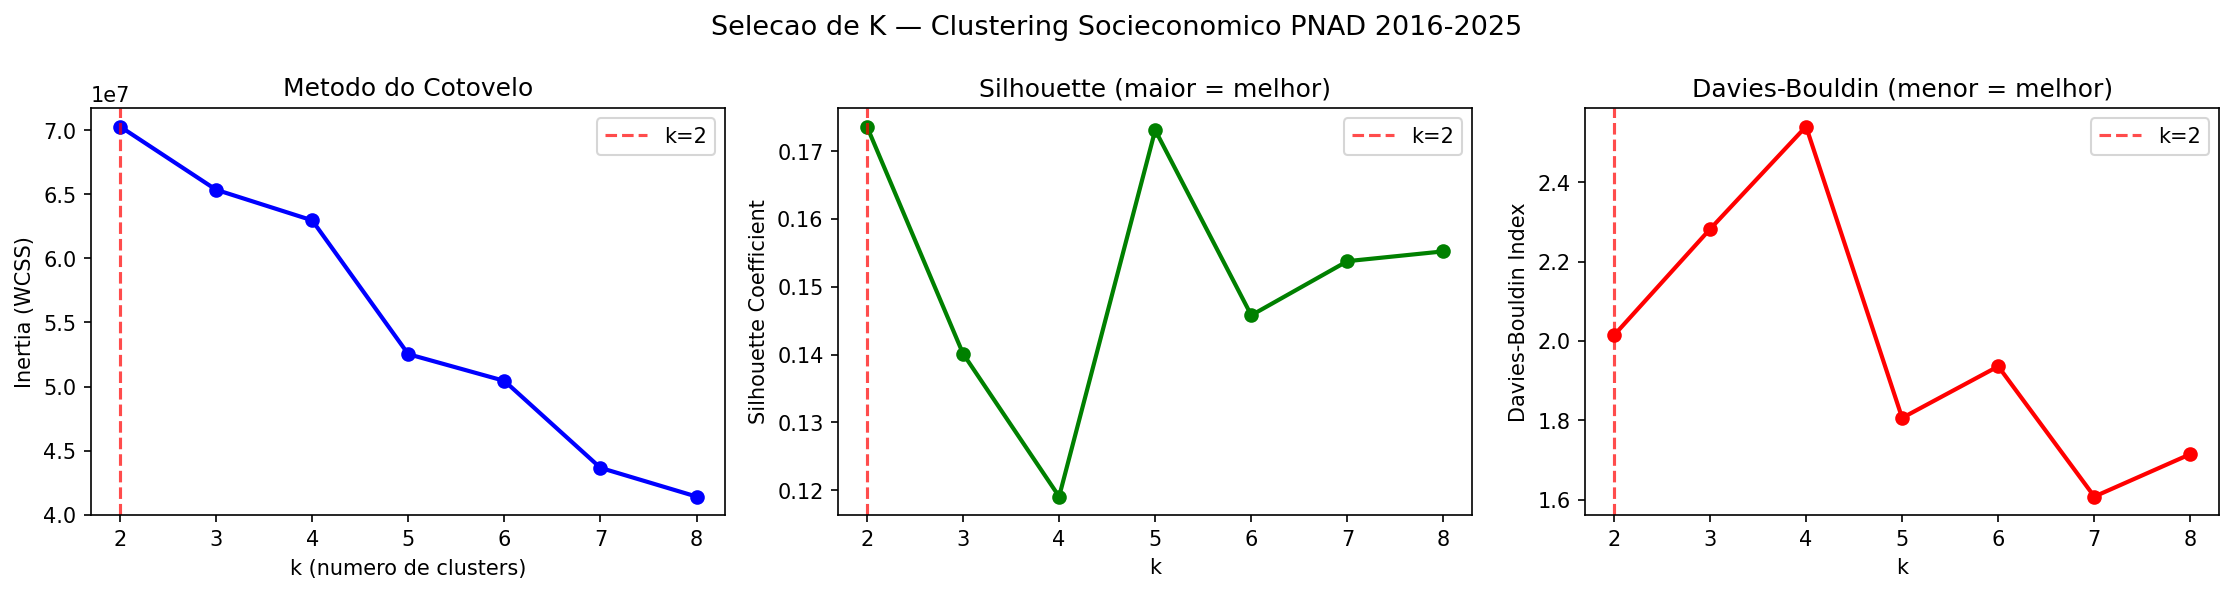
\includegraphics[width=\textwidth]{kmeans_selecao_k}
    \caption{Curvas de seleção de $k$: método do cotovelo,
              Silhouette e Davies-Bouldin.}
    \label{fig:kmeans_k}
  \end{subfigure}
  \hfill
  \begin{subfigure}[b]{0.49\textwidth}
    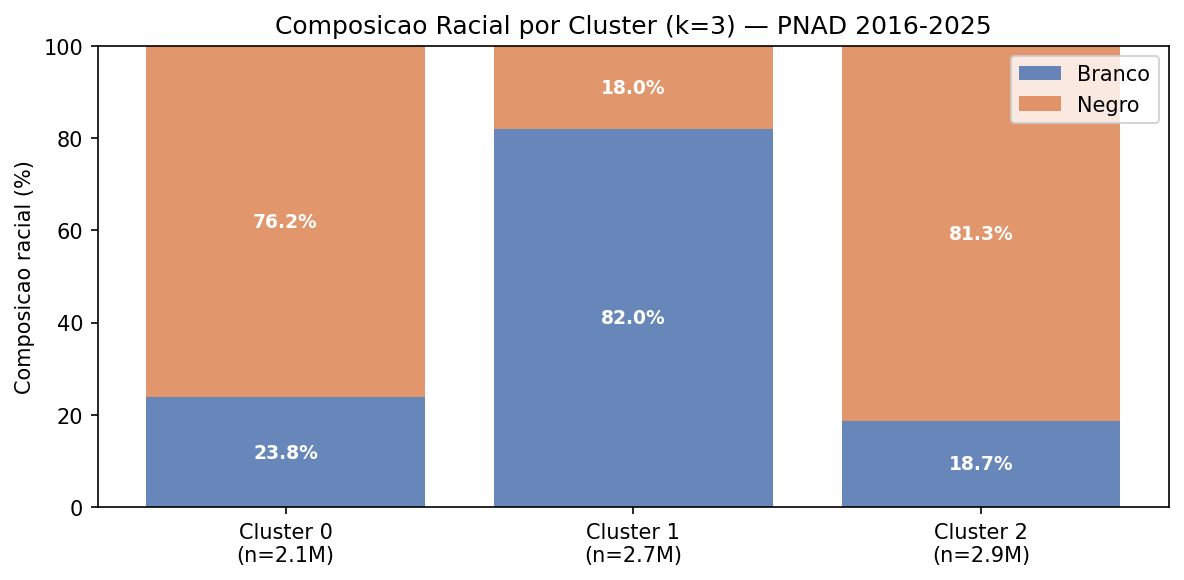
\includegraphics[width=\textwidth]{kmeans_composicao_racial_k3}
    \caption{Composição racial por cluster ($k=3$).}
    \label{fig:kmeans_raca}
  \end{subfigure}
  \caption{Clustering socioeconômico --- PNAD 2016--2025
            ($N=7{,}7$ milhões de trabalhadores da PEA completa).}
  \label{fig:kmeans}
\end{figure}

\subsection{M3 com Inclinação Aleatória de Negro: Heterogeneidade Geográfica}
\label{subsec:hlm_rs}

No modelo M3 padrão, $\hat{\beta}_1$ é constante entre estados.
Estimou-se M3 com \textit{random slope} para \texttt{negro} por UF
(população completa ($N=7.689.426$)),
testando $H_0{\colon}\,\tau^2_1 = 0$ (discriminação homogênea entre estados).

O LRT boundary test \cite{stram1994} rejeita $H_0$ com $LR=7547,7$, $p<0{,}001$: o gap racial varia significativamente entre estados. O efeito fixo nacional é $\hat{\beta}_1=−0,1206$ (gap de 11,4\%), com $\tau^2_1=0,002548$ ($DP=0,0505$ log-pontos). Em 95\% das UFs o gap situa-se em $[−19,7\%;\,−2,1\%]$ --- variação de 17,6 pontos percentuais entre extremos.

A correlação $\rho(u_0,u_1)=−0,367$ é negativa: UFs com maior nível salarial médio (intercepto $u_0$ mais alto) exibem penalidade racial mais severa (inclinação $u_1$ mais negativa). A discriminação se intensifica nas economias mais ricas e desiguais --- e não nas mais pobres: as maiores penalidades estimadas por UF concentram-se no Distrito Federal, Rio de Janeiro e São Paulo, ao passo que estados do Nordeste (RN, PB, SE) registram as menores ($r_{\text{UF}}=+0{,}45$ entre renda média e magnitude do gap).

\medskip
\noindent\textbf{Nível adicional --- gênero.} Estendendo o \textit{random slope} a \texttt{sexo\_fem} ($(1+\text{negro}+\text{sexo\_fem}\mid \text{UF})$), o LRT confirma que o gap salarial de gênero também varia geograficamente ($LR=15.584$, $p<0{,}001$) --- com \emph{maior} dispersão que o racial ($DP_{\text{gênero}}=0,064$ vs $DP_{\text{raça}}=0,049$ log-pontos). A correlação entre as duas inclinações é negativa ($\rho=−0,46$): nas UFs de maior penalidade racial, a de gênero tende a ser menor (discriminações geograficamente compensatórias).

\subsection{Random Slope no GLMM: Heterogeneidade Geográfica do Acesso}
\label{subsec:glmm_rs}

Estendeu-se o \textit{random slope} de \texttt{negro} ao GLMM logístico de acesso (\texttt{lme4::glmer}, população completa, $N=7.694.198$), em três desfechos. O LRT de fronteira rejeita $H_0{\colon}\,\tau^2_1=0$ em todos --- \texttt{ocp\_qualif} ($LR=2.406$), \texttt{y\_top20} ($LR=326$) e \texttt{y\_top10} ($LR=505$), todos $p<0{,}001$: a barreira de acesso também varia geograficamente. A heterogeneidade é maior no acesso a ocupações qualificadas ($\tau^2_1=0,0113$, $DP=0,106$ log-odds) e preserva o gradiente de teto de vidro no efeito fixo (OR cai de 0,707 para 0,662 rumo ao decil superior).

Em contraste com o salário ($\rho=-0{,}37$), o acesso a cargos qualificados correlaciona-se \emph{positivamente} com o nível ocupacional do estado ($\rho=0,65$): UFs com mais empregos qualificados exibem \emph{menor} penalidade de acesso --- nas economias desenvolvidas, negros enfrentam acesso relativamente mais fácil, porém maior gap salarial uma vez dentro.

\textbf{Setor público {\texttimes} privado.} A barreira de acesso é praticamente idêntica (OR$_{\text{púb}}=0,705$ vs OR$_{\text{priv}}=0,698$) e igualmente heterogênea entre UFs ($\tau^2=0,0115$ vs $0,0109$): o concurso público \emph{não dissolve} a exclusão racial de acesso a ocupações qualificadas.

\begin{figure}[H]
  \centering
  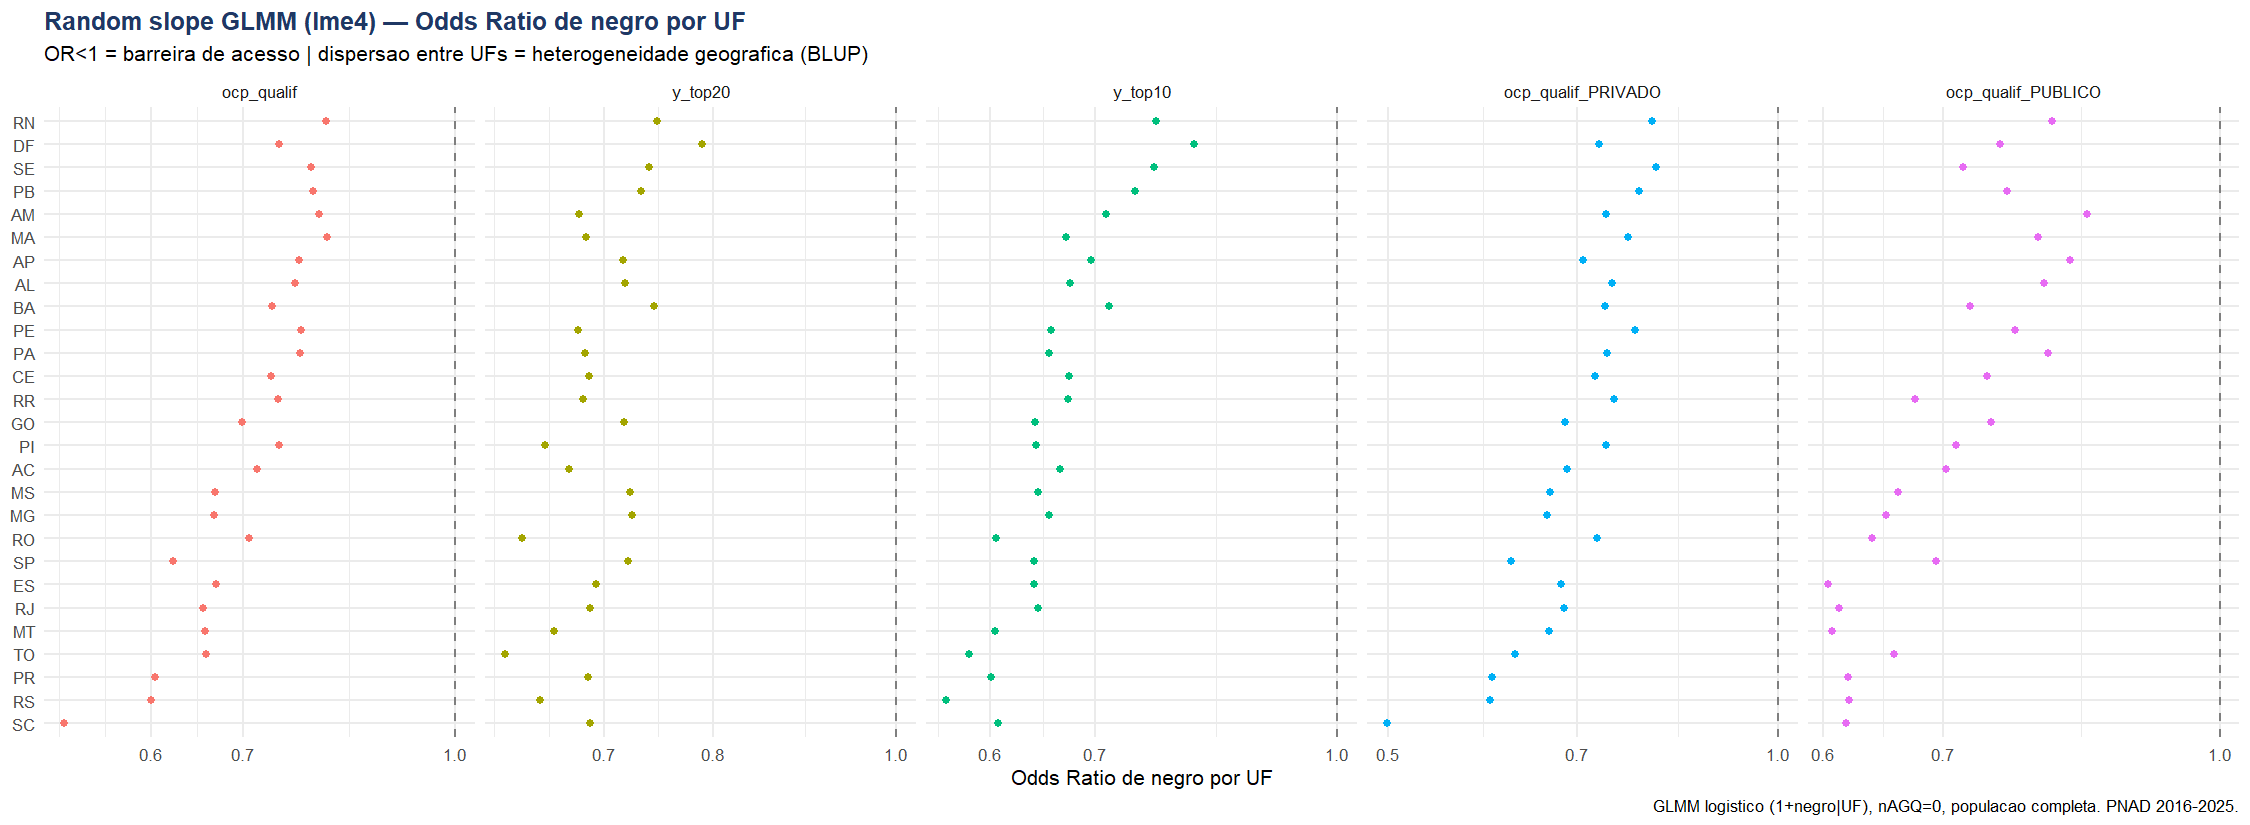
\includegraphics[width=\textwidth]{outputs/figures/glmm_rs_real.png}
  \caption{Random slope GLMM (\texttt{lme4}): Odds Ratio de \texttt{negro} por UF em cada desfecho de acesso e por setor. Dispersão entre UFs = heterogeneidade geográfica (BLUP); OR$<$1 = barreira.}
  \label{fig:glmm_rs}
\end{figure}


Já no \emph{salário}, o setor público \emph{atenua} o gap racial (7,7\% vs 11,1\% no privado) e o \emph{homogeneíza} entre UFs ($\tau^2_1=0,00140$ vs $0,00217$). O concurso equaliza a \emph{remuneração} de quem entra, mas não a \emph{entrada} --- precisando o diagnóstico ``o Estado ajuda, mas não resolve''.

\medskip
\noindent\textbf{Gênero no acesso.} O mesmo \textit{random slope} aplicado a \texttt{sexo\_fem} no GLMM confirma heterogeneidade geográfica em todos os desfechos ($p<0{,}001$), revelando uma divergência ausente no caso racial: mulheres têm \emph{mais} acesso a ``ocupações qualificadas'' (OR$=1,99>1$, por profissões credenciadas feminizadas), mas \emph{muito menos} acesso ao topo da renda (OR$_{\text{top20}}=0,562$; OR$_{\text{top10}}=0,518$). O teto de vidro de gênero é de \emph{remuneração}, não de categoria ocupacional --- e sua heterogeneidade geográfica supera a racial no topo ($\tau^2_{\text{sexo}}=0,0323$ no top20, contra $\tau^2_{\text{negro}}\approx0{,}003$; cerca de 10$\times$).

\begin{figure}[H]
  \centering
  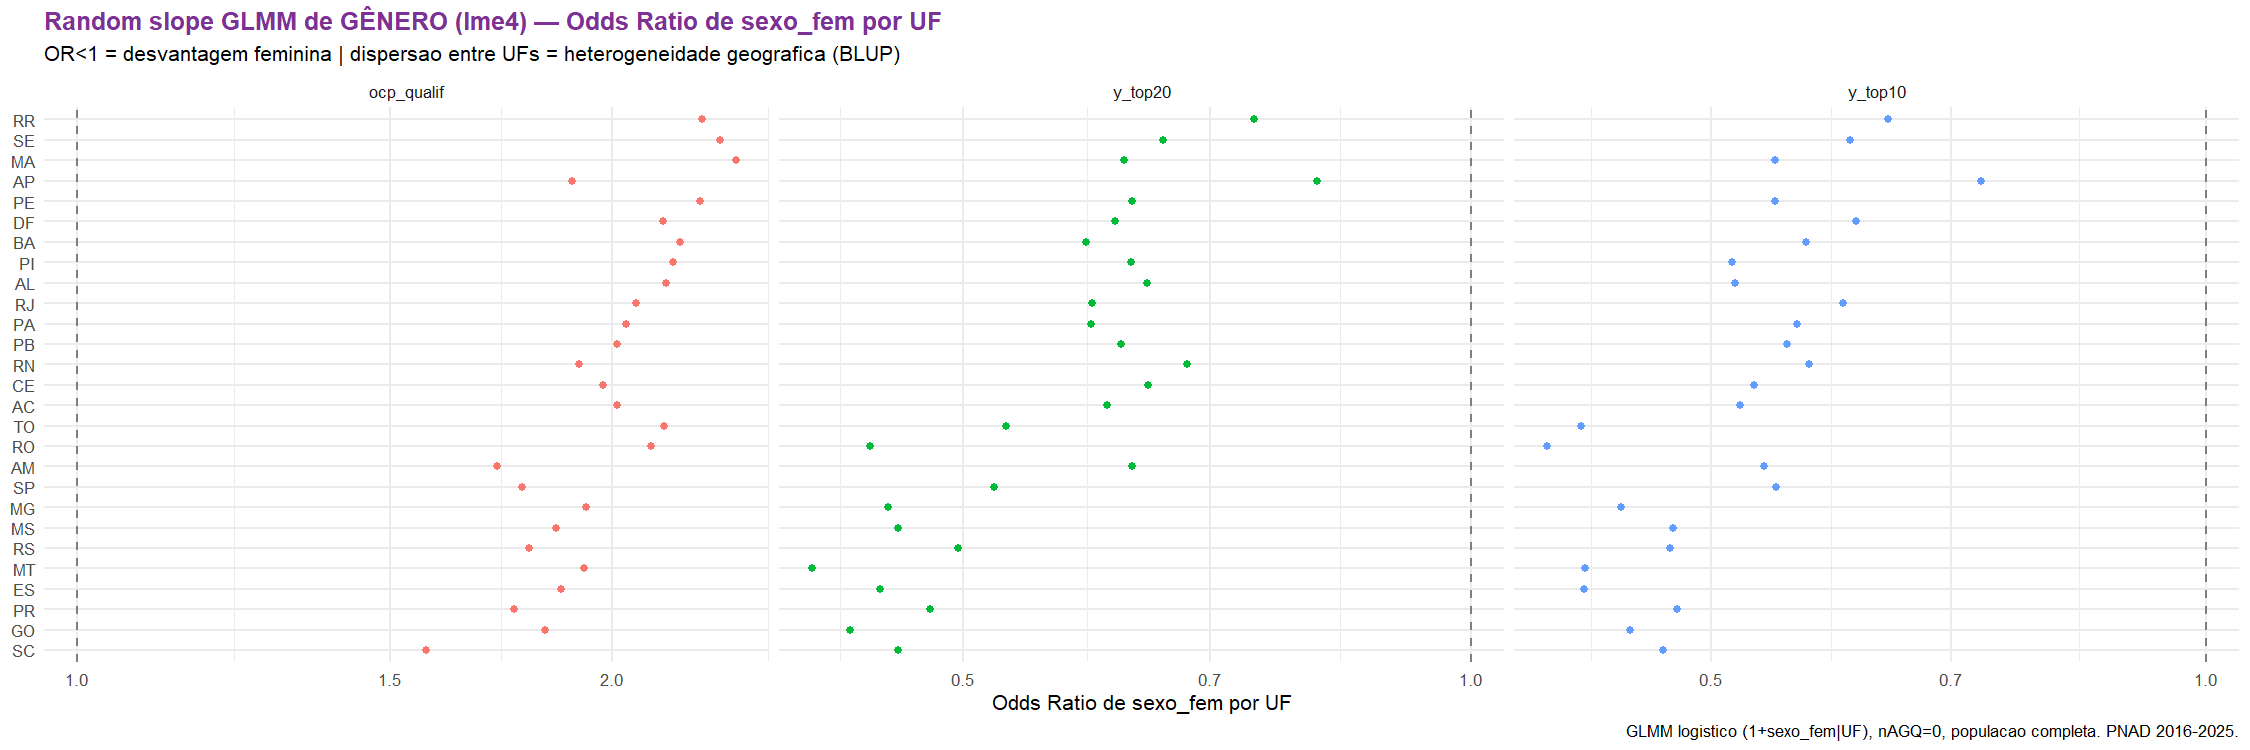
\includegraphics[width=\textwidth]{outputs/figures/glmm_genero_real.png}
  \caption{Random slope GLMM de gênero (\texttt{lme4}): OR de \texttt{sexo\_fem} por UF em cada desfecho. OR$>$1 = vantagem feminina na categoria; OR$<$1 = desvantagem na renda (teto de vidro de remuneração).}
  \label{fig:glmm_genero}
\end{figure}


\noindent\rule{\textwidth}{1pt}
\textbf{\large BARREIRA II --- PENALIDADE RESIDUAL E TETO DE VIDRO}
\textit{O custo de ser negro, mesmo após superar a barreira de entrada}
\noindent\rule{\textwidth}{1pt}

\medskip

\textit{Estabelecida a exclusão de acesso (Barreira I), a próxima questão é:
para os trabalhadores negros que superam essa barreira --- qual é a penalidade
salarial residual? E como esse custo evolui à medida que sobem na distribuição?}

\subsection{Clustering Socioeconômico}
\label{subsec:clustering}

Os critérios automáticos apresentam divergência esperada:
$k=2$ ($S=0.1736$, $DB=2,0140$) produz
clusters mais compactos; $k=3$ ($S=0.1401$,
$DB=2,2814$) foi adotado por interpretabilidade substantiva
\cite{ketchen1996}, uma vez que a solução binária reproduz trivialmente a
clivagem racial sem discriminar segmentos ocupacionais internos
(Figura~\ref{fig:kmeans}). A Tabela~\ref{tab:kmeans_perfis} apresenta os
perfis médios por cluster.

\begin{table}[H]
\centering
\caption{Perfis dos Clusters Socioeconômicos ($k=3$) --- PNAD 2016--2025.
          $N=7{,}7$ milhões de trabalhadores da PEA completa.}
\label{tab:kmeans_perfis}
\begin{tabular}{lccccccc}
\toprule
\textbf{Cluster} & \textbf{N} & \textbf{\%} & \textbf{\%~Negro} &
\textbf{\%~Mulher} & \textbf{log\_Renda} & \textbf{Descrição} \\
\midrule
C0 & 2.110.270 & 27,4\% & 76,2\%  & 100\% & 6,961 &
  Mulheres negras --- vulnerabilidade dupla \\
C1 & 2.705.788 & 35,2\% & 18,0\%  & \phantom{0}40,1\%  & 7,895 &
  Brancos --- alta renda, menor escolaridade \\
C2 & 2.878.140 & 37,4\% & 81,3\%  & \phantom{00}0\% & 7,074 &
  Homens negros --- maior escolaridade, renda inferior \\
\bottomrule
\end{tabular}
\end{table}

O Cluster~0 concentra mulheres negras (76,2\% negras,
100\% feminino), com rendimento médio de
R\$1.447 ($\log=6,961$) e
21,7\% com ensino superior.
O Cluster~1 agrupa predominantemente brancos (82\% não negros)
com o maior rendimento do conjunto --- R\$3.830
($\log=7,895$) ---
e apenas 13,7\% com superior completo.

O Cluster~2 reúne homens negros (81,3\% negros,
0\% feminino) com
$\log\text{-renda}=7,074$ e 36,5\%
com superior completo: escolaridade quase três vezes maior que o Cluster~1,
porém com rendimento 58\%
inferior, evidenciando a dupla desvantagem de gênero e raça
(Hipótese~H3) e confirmando que o capital humano é subconvertido em renda
para trabalhadores negros (Hipótese~H5).

\subsection{Modelos de Machine Learning e SHAP Values}
\label{subsec:ml}

A Tabela~\ref{tab:ml_perf} apresenta o desempenho preditivo dos dois modelos
sobre o conjunto de teste (\textit{hold-out} 20\%).

\begin{table}[H]
\centering
\caption{Desempenho preditivo --- Random Forest e XGBoost.
          \textit{Hold-out} 20\%, $N_\text{teste}=307.768$ observações.}
\label{tab:ml_perf}
\begin{tabular}{lccc}
\toprule
\textbf{Modelo} & $R^2$ & \textbf{MAE} & \textbf{RMSE} \\
\midrule
Random Forest  & 0.5743  & 0.4283 & --- \\
\textbf{XGBoost}      & \textbf{0.6169} & \textbf{0.4283} & \textbf{0,6986} \\
\bottomrule
\end{tabular}
\end{table}

O $R^2 \approx 0{,}43$ é robusto para dados de rendimento individual,
onde a variância não observada (setor, cargo, tempo de serviço) responde
pela maior parte do resíduo.

\begin{table}[H]
\centering
\caption{Importância SHAP Comparada --- Random Forest e XGBoost. Predição de log-rendimento, PNAD 2016--2025 ($N_{\text{SHAP}}=50.000$). Valores: $|\text{SHAP}|$ médio. Destaque em negrito: variáveis raciais/contextuais.}
\label{tab:shap_importance}
\begin{tabular}{lcccc}
\toprule
\textbf{Feature} & \textbf{$|\text{SHAP}|$ RF} & \textbf{Rank RF} & \textbf{$|\text{SHAP}|$ XGB} & \textbf{Rank XGB} \\
\midrule
\textbf{Renda média UPA} & 0.32872 & 1 & 0.26938 & 1 \\
Horas trabalhadas & 0.17613 & 2 & 0.16362 & 2 \\
CBO: Profissionais & 0.11208 & 4 & 0.11665 & 3 \\
Emprego formal (carteira) & 0.13965 & 3 & 0.11006 & 4 \\
Gênero (feminino) & 0.09079 & 5 & 0.10083 & 5 \\
Idade (centralizada) & 0.06466 & 6 & 0.10055 & 6 \\
Educ.: não registrada & 0.02108 & 9 & 0.07063 & 7 \\
Conta própria & 0.02049 & 10 & 0.06345 & 8 \\
CBO: Técnicos & 0.03577 & 8 & 0.04579 & 9 \\
CBO: Dirigentes & 0.03673 & 7 & 0.03903 & 10 \\
\textbf{Raça (negro)} & 0.00033 & 23 & 0.02940 & 11 \\
CBO: Serviços/Vendas & 0.00121 & 16 & 0.02915 & 12 \\
\textbf{Desemprego na UPA} & 0.00152 & 15 & 0.02291 & 13 \\
CBO: Operários & 0.00068 & 18 & 0.02181 & 14 \\
CBO: Op. Máquinas & 0.00043 & 21 & 0.02057 & 15 \\
Trabalho doméstico & 0.00516 & 12 & 0.01853 & 16 \\
\textbf{\% Negro no Estado} & 0.00067 & 19 & 0.01838 & 17 \\
CBO: Administrativo & 0.00283 & 14 & 0.01773 & 18 \\
\textbf{Desemprego no Estado} & 0.00042 & 22 & 0.01531 & 19 \\
CBO: Agropecuária & 0.00117 & 17 & 0.01510 & 20 \\
CBO: FFAA/Polícia & 0.01083 & 11 & 0.01276 & 21 \\
Idade² (experiência) & 0.00507 & 13 & 0.01153 & 22 \\
\textbf{\% Negro na UPA} & 0.00033 & 23 & 0.01145 & 23 \\
Educ. média UPA & 0.00032 & 25 & 0.01099 & 24 \\
Educ. média Estado & 0.00054 & 20 & 0.00613 & 25 \\
Educ.: Médio & 0.00000 & 28 & 0.00402 & 26 \\
Educ.: Superior & 0.00002 & 26 & 0.00258 & 27 \\
Educ.: Fundamental & 0.00000 & 28 & 0.00104 & 28 \\
Educ.: Pós-graduação & 0.00000 & 28 & 0.00002 & 29 \\
\bottomrule
\end{tabular}
\end{table}

\begin{figure}[H]
  \centering
  \begin{subfigure}[b]{0.49\textwidth}
    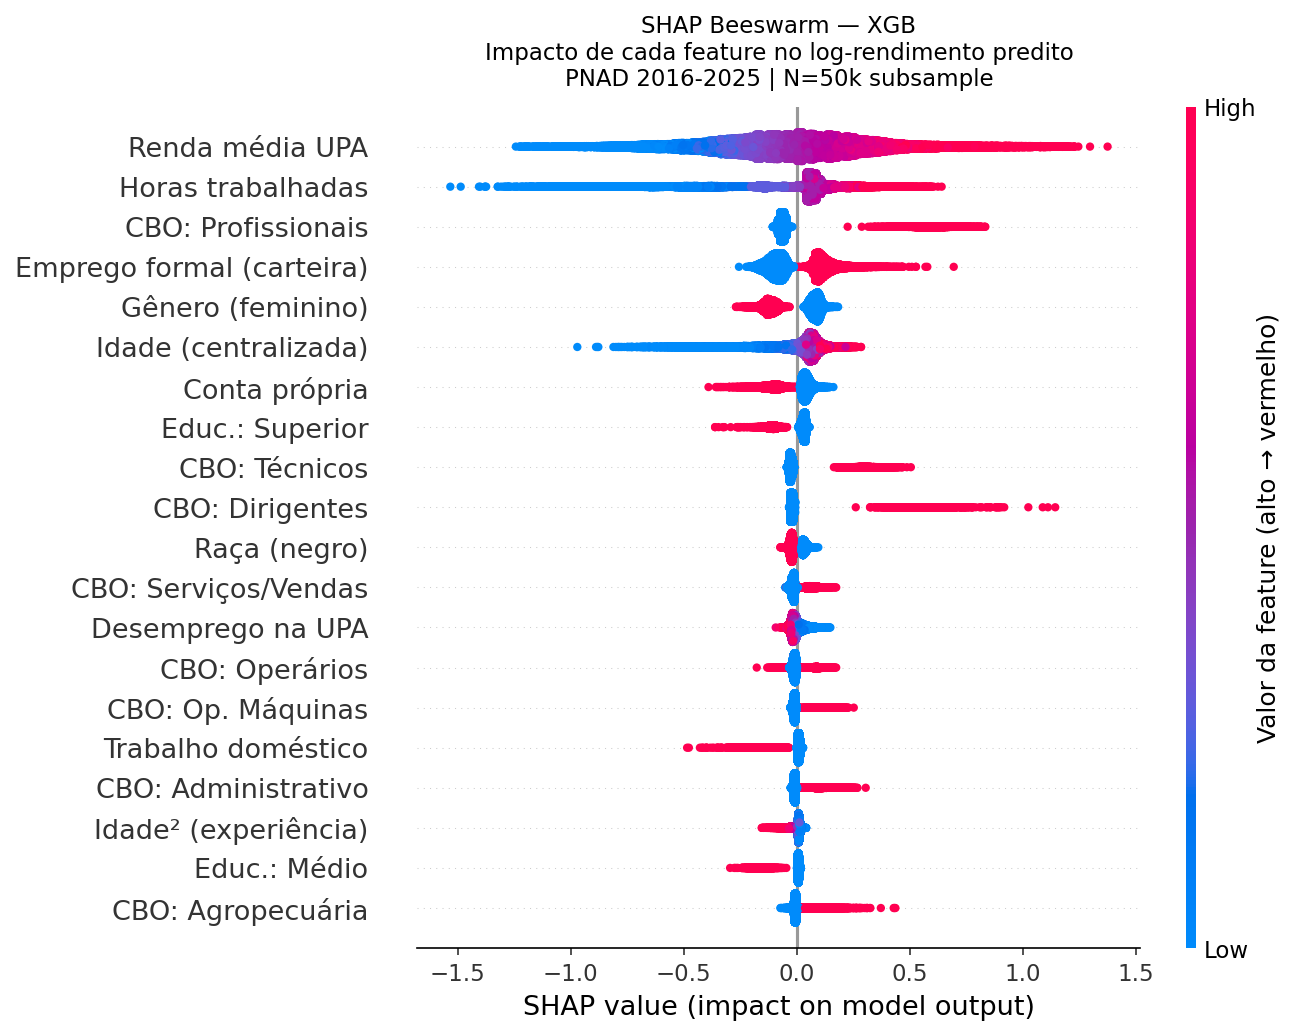
\includegraphics[width=\textwidth]{shap_beeswarm_xgb}
    \caption{Beeswarm: distribuição de SHAP por feature (XGBoost).}
    \label{fig:shap_bee}
  \end{subfigure}
  \hfill
  \begin{subfigure}[b]{0.49\textwidth}
    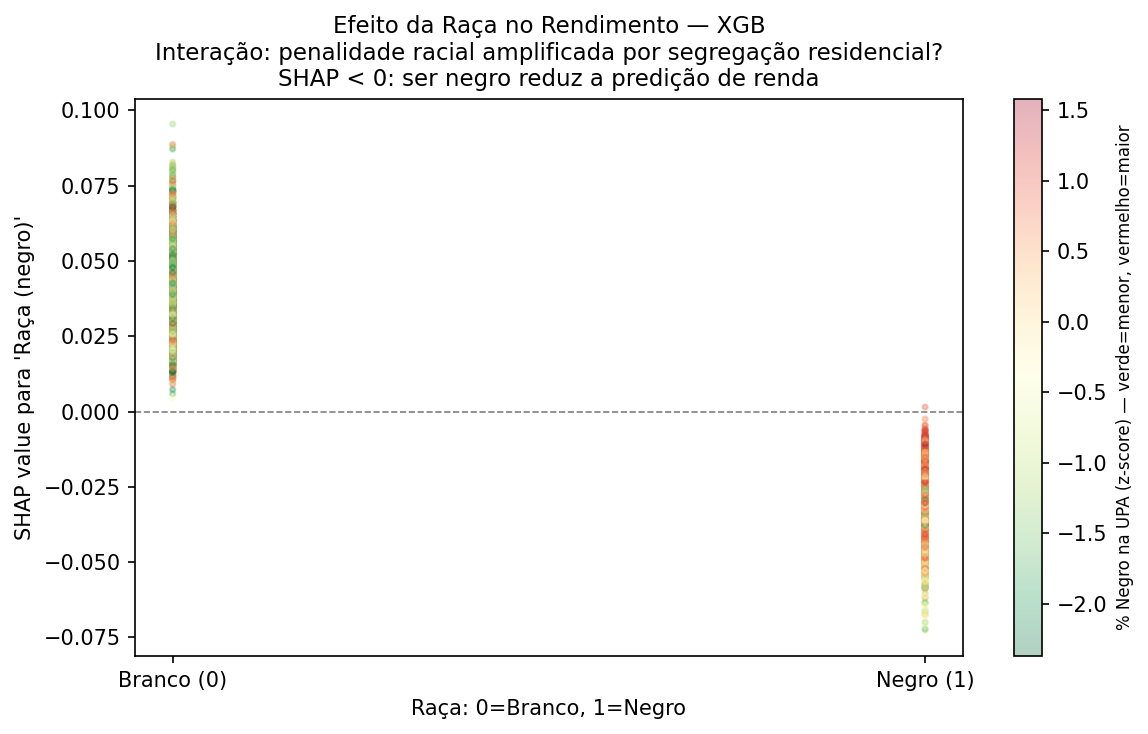
\includegraphics[width=\textwidth]{shap_dependence_negro_xgb}
    \caption{Dependence plot: efeito da raça colorido por
              \% negro na UPA (interação contextual).}
    \label{fig:shap_dep}
  \end{subfigure}
  \caption{Análise SHAP --- XGBoost ($N_\text{SHAP}=50.000$).}
  \label{fig:shap}
\end{figure}

A Tabela~\ref{tab:shap_importance} revela que a \textbf{renda média da UPA}
é o preditor mais importante do rendimento individual
($|\text{SHAP}| = 0.269$), com peso três vezes maior que
a escolaridade superior e 2,5 vezes maior que o gênero.
Esse resultado confirma computacionalmente a hipótese de Wilson~(\citeyear{wilson1987}):
o \textit{onde se mora} supera em importância o \textit{quanto se estudou}.

A variável racial ocupa o 11$^\circ$ lugar no ranking de
importância mesmo após controlar por todos os demais fatores, com SHAP
médio de $-0{,}0469$ para trabalhadores negros --- equivalente a uma
penalidade de 4,6\% sobre o rendimento predito que não pode ser atribuída
a diferenças em educação, experiência, gênero ou contexto de moradia.

\begin{figure}[H]
  \centering
  \begin{subfigure}[b]{0.32\textwidth}
    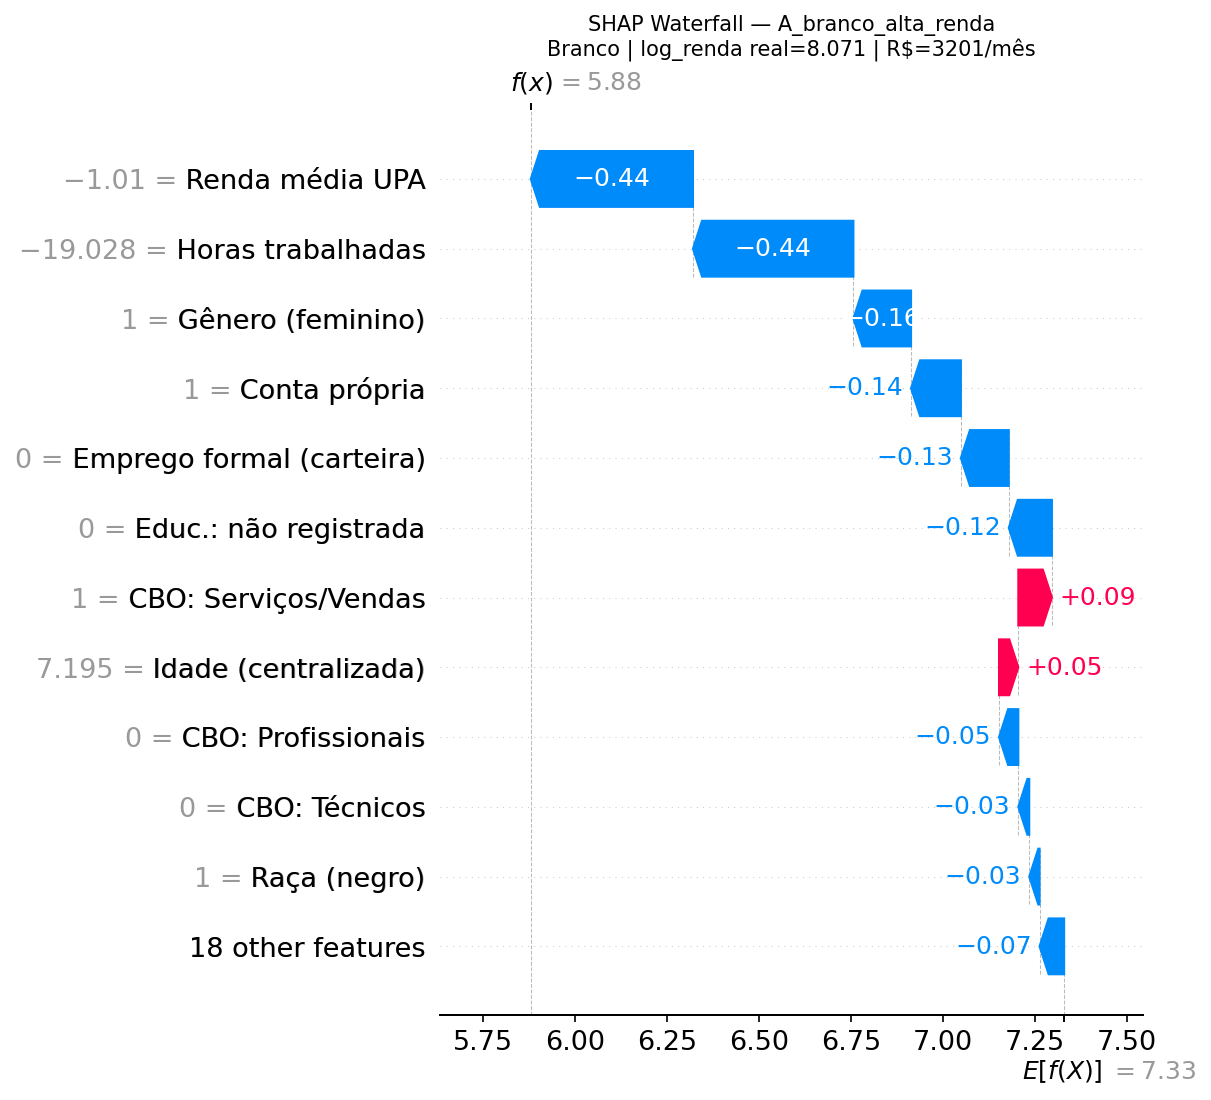
\includegraphics[width=\textwidth]{shap_waterfall_A_branco_alta_renda_xgb}
    \caption{Caso A: branco de alta renda.}
  \end{subfigure}
  \hfill
  \begin{subfigure}[b]{0.32\textwidth}
    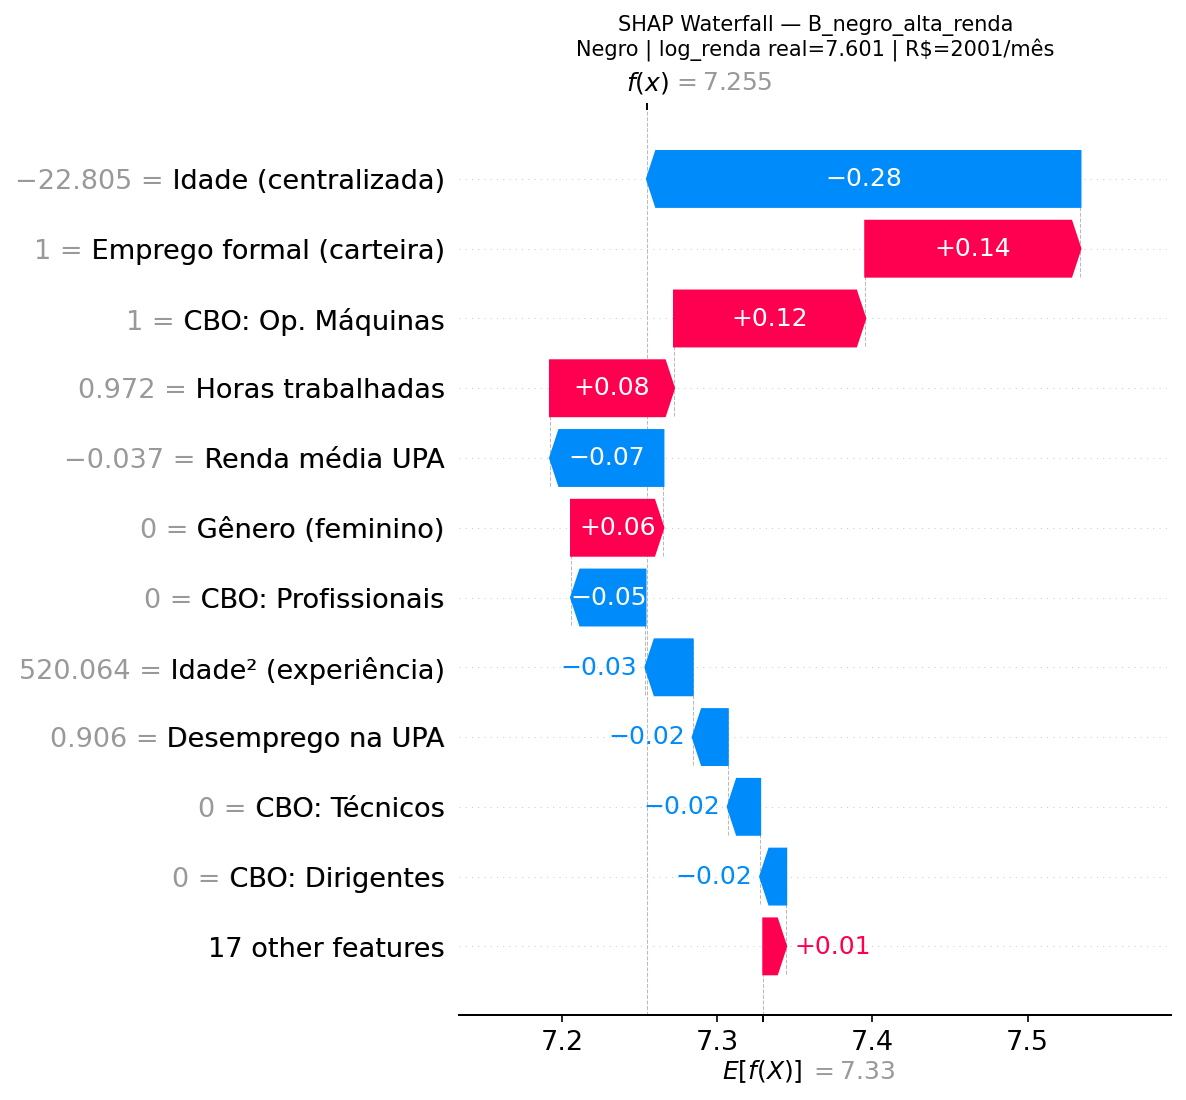
\includegraphics[width=\textwidth]{shap_waterfall_B_negro_alta_renda_xgb}
    \caption{Caso B: negro de alta renda.}
  \end{subfigure}
  \hfill
  \begin{subfigure}[b]{0.32\textwidth}
    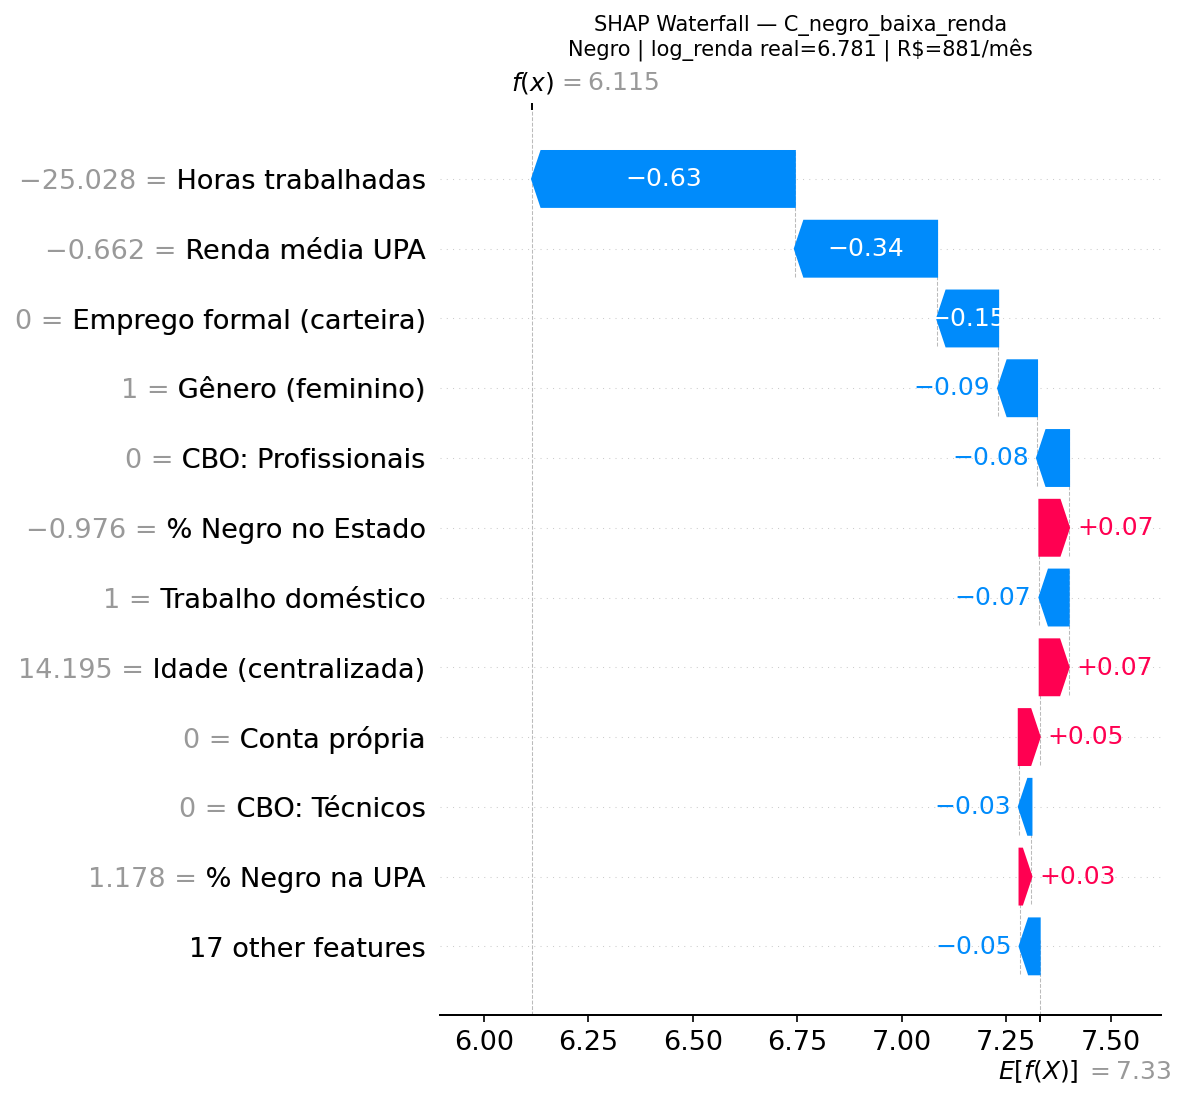
\includegraphics[width=\textwidth]{shap_waterfall_C_negro_baixa_renda_xgb}
    \caption{Caso C: negro de baixa renda.}
  \end{subfigure}
  \caption{Decomposição SHAP individual (waterfall) para três perfis representativos.
            Valores em log-pontos; azul = contribuição positiva, vermelho = negativa.}
  \label{fig:shap_wf}
\end{figure}

\subsection{Interseccionalidade: raça e gênero no acesso e no topo}
\label{subsec:interseccional}

Os modelos anteriores tratam raça e gênero de forma aditiva. Uma leitura
\textit{interseccional} pergunta se a desvantagem de ser negra \emph{e} mulher é a
soma das partes. Reespecificamos o GLMM de acesso com um fator de quatro grupos
(\texttt{grupo\_rg}: homem branco [referência], mulher branca, homem negro, mulher
negra) e a interação \texttt{negro$\times$sexo\_fem}, em três desfechos: acesso a
ocupação qualificada (CBO~1--4), renda no top~20\% e no top~10\%.

\begin{figure}[htbp]
  \centering
  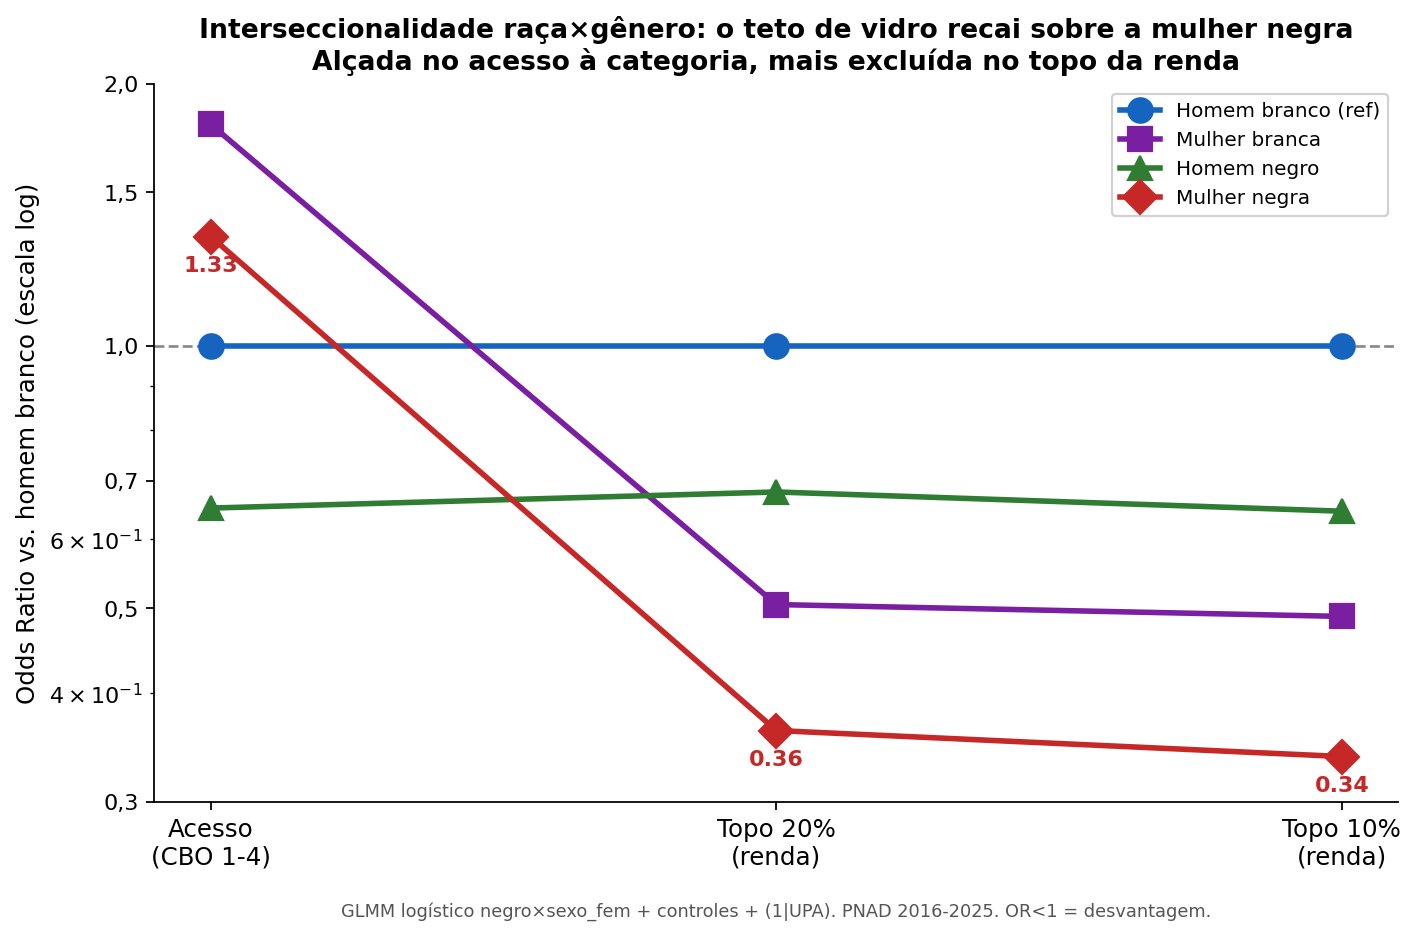
\includegraphics[width=0.82\textwidth]{grupo_rg_interseccional}
  \caption{Razões de chance dos quatro grupos raça$\times$gênero \textit{vs.}~homem
  branco, em três desfechos. A mulher negra é \emph{alçada} no acesso à categoria,
  mas torna-se a \emph{mais excluída} no topo da renda.}
  \label{fig:interseccional}
\end{figure}

O resultado revela uma \textbf{inversão} (Figura~\ref{fig:interseccional}). No
\textbf{acesso à categoria} qualificada, a mulher negra tem OR~$=1,33$
--- \emph{acima} do homem branco ---, porque o efeito de gênero é positivo nesse
desfecho (profissões credenciadas feminizadas, em CBO~1--4); o grupo mais penalizado
é o \textbf{homem negro} (OR~$=0,65$). No \textbf{topo da renda},
porém, o quadro \emph{inverte}: a mulher negra passa a ser a \textbf{mais excluída}
de todos --- OR~$=0,34$ no decil superior, abaixo da mulher branca
($=0,49$) e do homem negro ($=0,65$). A
interação \texttt{negro$\times$sexo\_fem} é \textit{sub-aditiva} em todos os desfechos
(OR~$=1,14$ no acesso; $=1,07$ no top~10\%):
a penalidade racial é ligeiramente menor entre mulheres, mas isso não impede que a
mulher negra acumule a barreira racial \emph{e} o teto de vidro de gênero exatamente
onde mais importa para a ascensão --- o topo da distribuição.

Esse achado refina a tese central: o teto de vidro não é racial nem sexualmente neutro
--- recai com força máxima sobre a mulher negra, que pode \emph{entrar} em ocupações
qualificadas, mas é sistematicamente barrada de \emph{chegar ao topo} da remuneração.

\noindent\rule{\textwidth}{1pt}
\textbf{\large BARREIRA III --- ISOLAMENTO ESTRUTURAL E CAPITAL SOCIAL}
\textit{Por que educação, sozinha, não quebra o ciclo}
\noindent\rule{\textwidth}{1pt}

\medskip

\textit{As barreiras anteriores documentam exclusão mensurável por econometria.
Esta seção documenta o mecanismo que as sustenta: o isolamento estrutural
das redes de capital social, que explica por que trabalhadores negros com
pós-graduação ainda não chegam ao topo.}

\subsection{Análise de Redes Sociais --- Isolamento Estrutural}
\label{subsec:sna}

\begin{table}[H]
\centering
\caption{Métricas de Rede por Grupo Demográfico (Raça $\times$ Educação). PNAD 2016--2025. \textit{Constraint} de Burt: maior valor = maior isolamento estrutural. \textit{Betweenness}: capacidade de corretagem entre grupos.}
\label{tab:sna_metricas}
\begin{tabular}{llllcccc}
\toprule
\textbf{Grupo} & \textbf{Raça} & \textbf{Educação} & \textbf{N} & \textbf{log\_Renda} & \textbf{Betweenness} & \textbf{Constraint} \\
\midrule
Branco\_Sem\_Instr & Branco & Sem\_Instr & 4,378,114 & 7.729 & 0.000 & 0.4238 \\
Branco\_Fundamental & Branco & Fundamental & 57,697 & 6.559 & \textbf{0.306} & 0.4177 \\
Branco\_Medio & Branco & Medio & 711,014 & 7.086 & 0.000 & 0.4228 \\
Branco\_Superior & Branco & Superior & 1,194,442 & 7.174 & 0.000 & 0.4209 \\
Branco\_Pos & Branco & Pos & 41,357 & 7.043 & \textbf{0.111} & 0.4220 \\
Negro\_Sem\_Instr & Negro & Sem\_Instr & 6,015,628 & 7.316 & 0.000 & 0.4236 \\
Negro\_Fundamental & Negro & Fundamental & 191,988 & 6.297 & 0.000 & 0.4156 \\
Negro\_Medio & Negro & Medio & 765,906 & 6.758 & 0.000 & 0.4191 \\
Negro\_Superior & Negro & Superior & 2,484,813 & 6.865 & 0.000 & 0.4210 \\
Negro\_Pos & Negro & Pos & 100,716 & 6.725 & 0.000 & 0.4152 \\
\bottomrule
\end{tabular}
\end{table}

\begin{figure}[H]
  \centering
  \begin{subfigure}[b]{0.49\textwidth}
    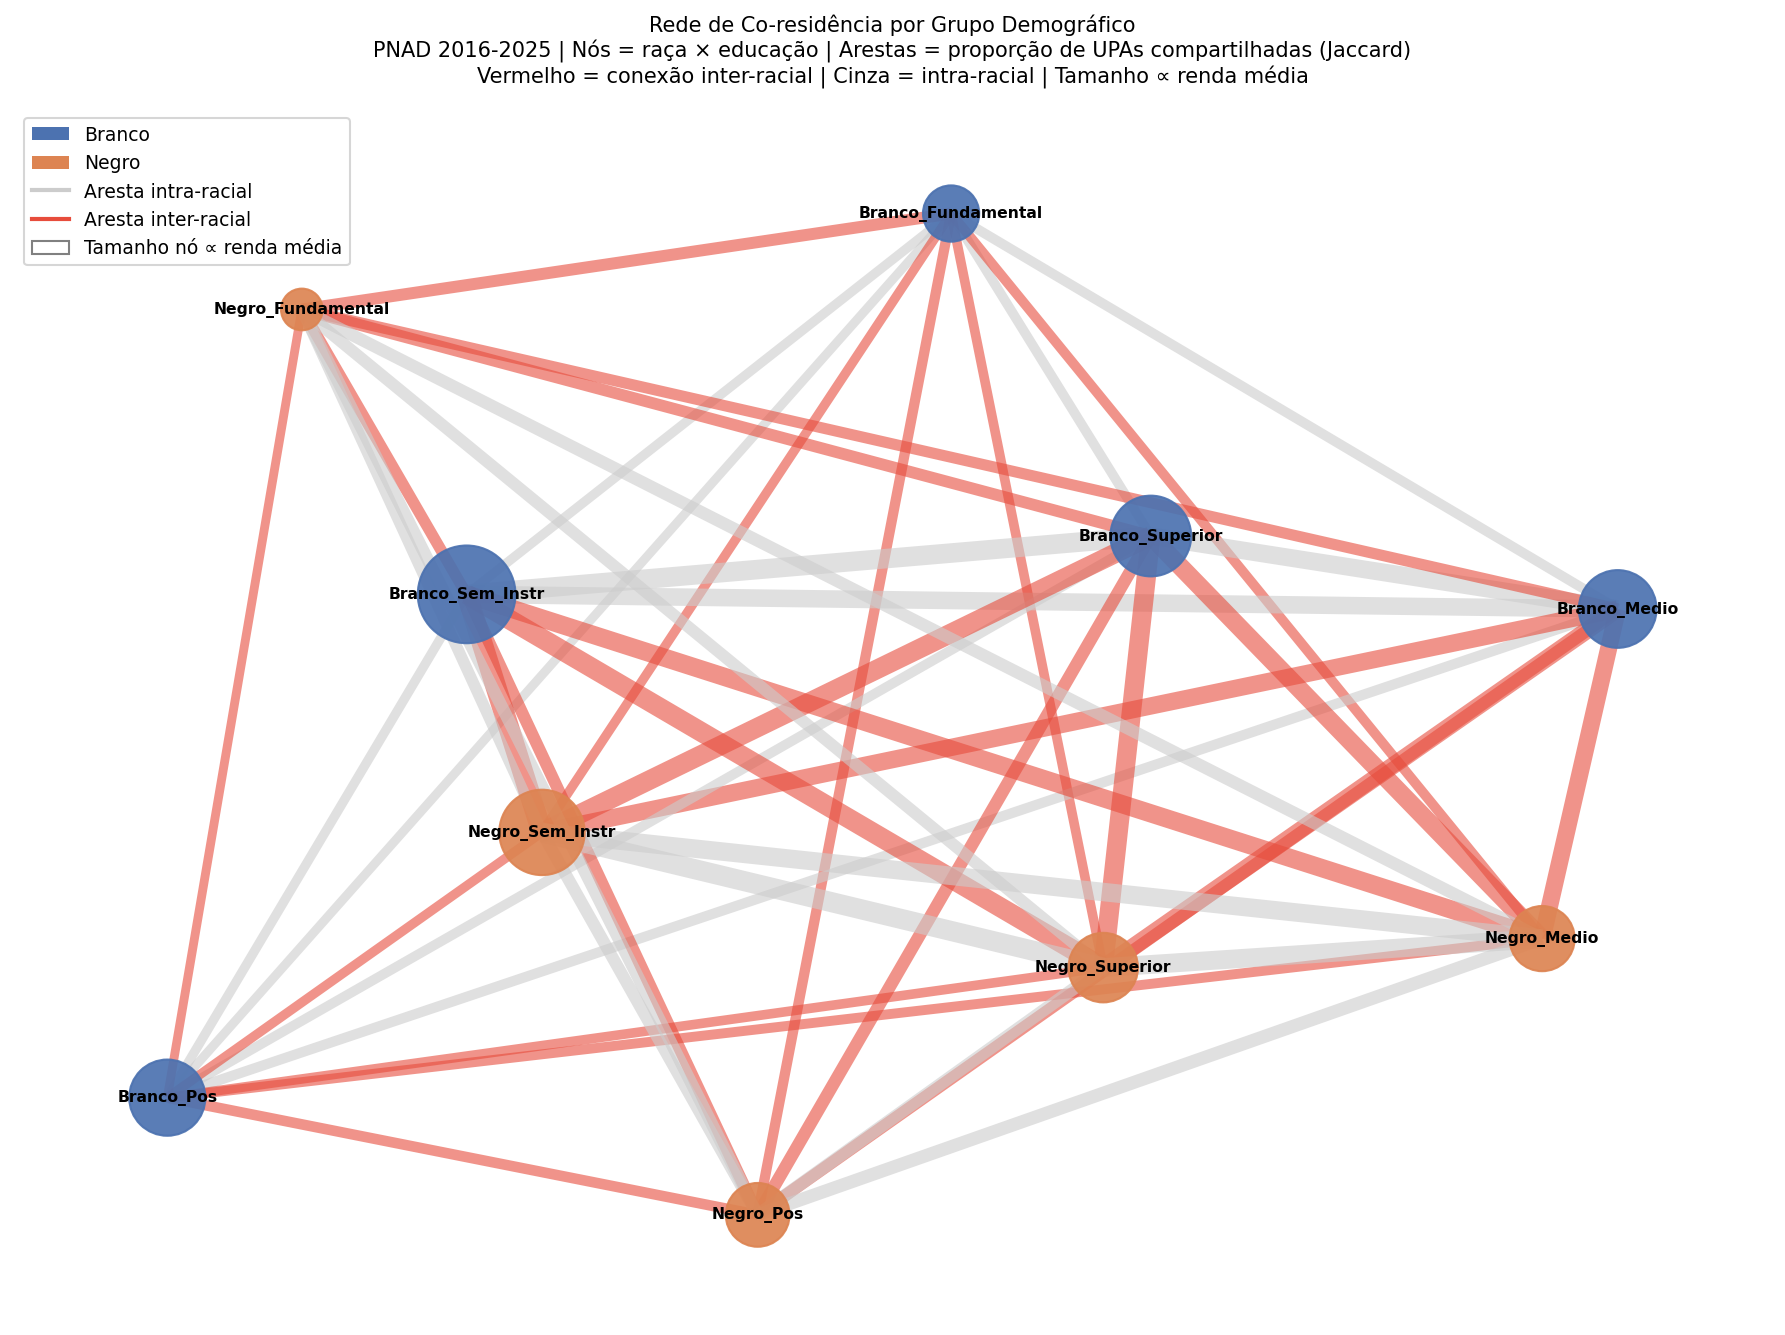
\includegraphics[width=\textwidth]{sna_rede_demografica}
    \caption{Grafo de co-residência: tamanho $\propto$ renda,
              vermelho = arestas inter-raciais.}
    \label{fig:sna_grafo}
  \end{subfigure}
  \hfill
  \begin{subfigure}[b]{0.49\textwidth}
    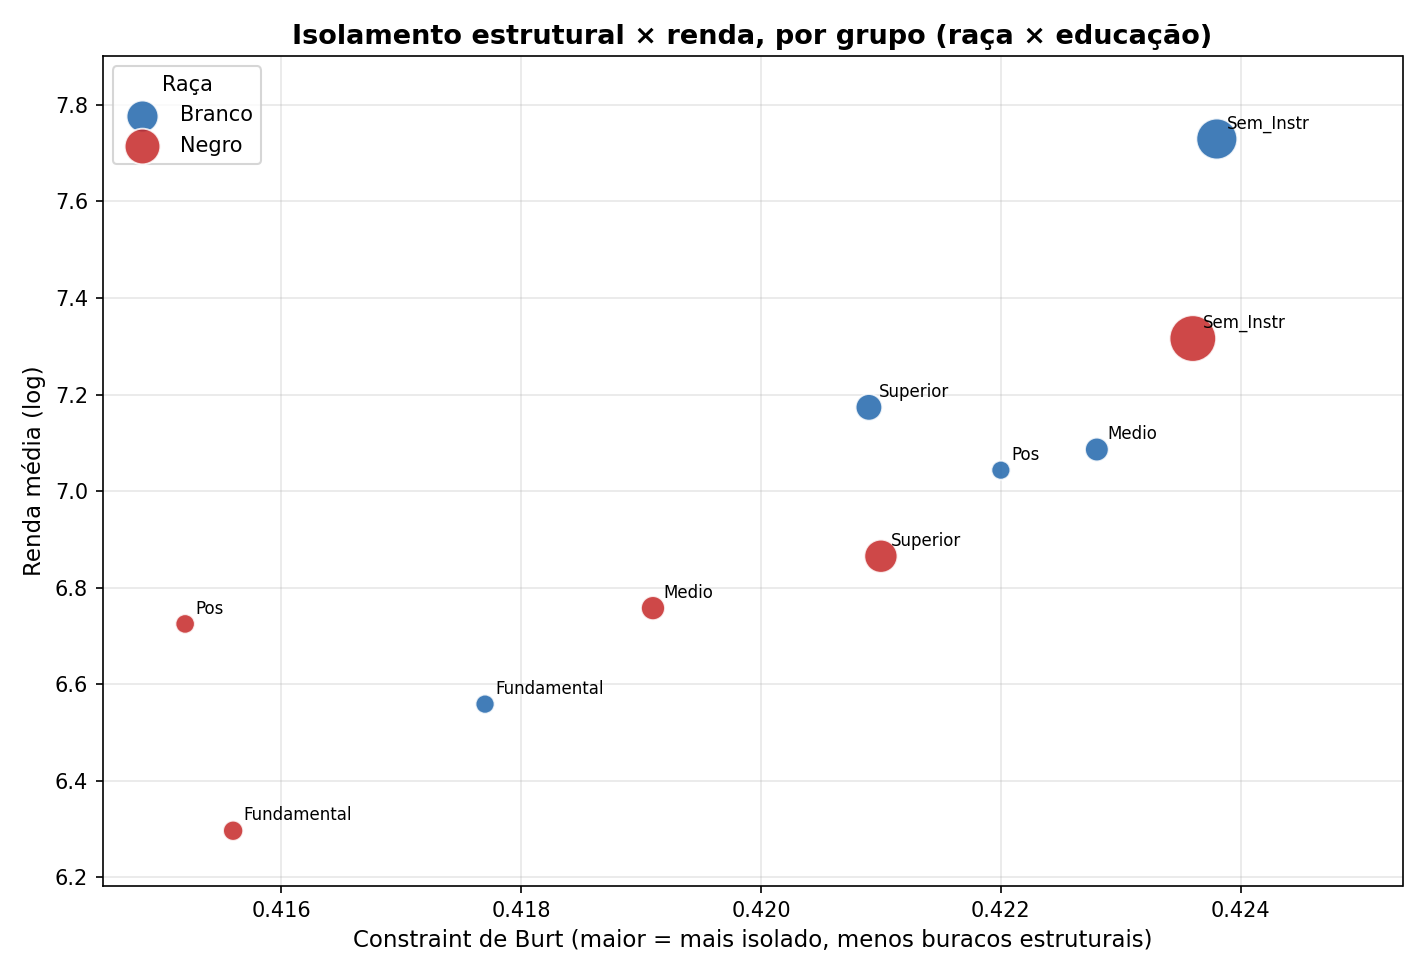
\includegraphics[width=\textwidth]{sna_constraint_vs_renda}
    \caption{Constraint de Burt $\times$ rendimento médio.}
    \label{fig:sna_constraint}
  \end{subfigure}
  \caption{Análise de Redes Sociais --- PNAD 2016--2025.
            Nós = raça $\times$ educação; arestas = índice Jaccard de co-presença em UPAs.}
  \label{fig:sna}
\end{figure}

\begin{figure}[H]
  \centering
  \begin{subfigure}[b]{0.49\textwidth}
    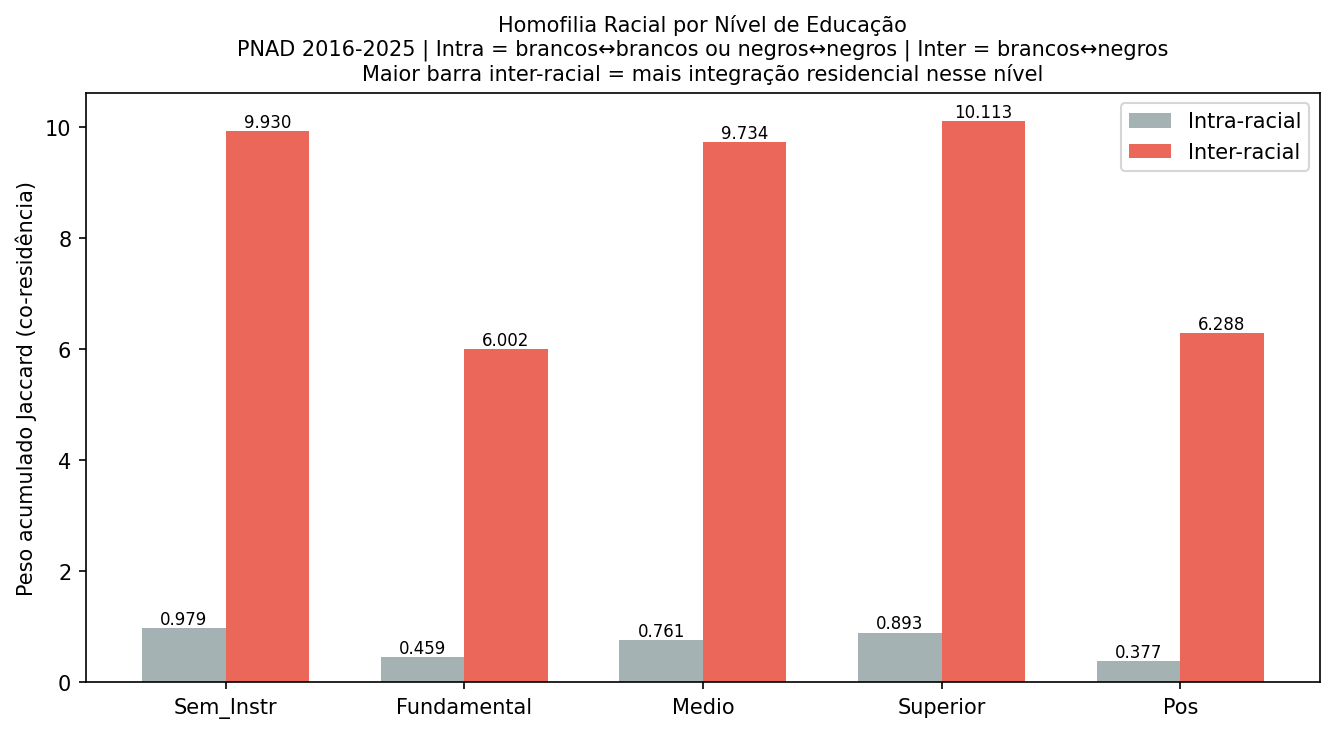
\includegraphics[width=\textwidth]{sna_homofilia_por_educ}
    \caption{Peso Jaccard intra vs.\ inter-racial por nível de educação.}
    \label{fig:sna_hom}
  \end{subfigure}
  \hfill
  \begin{subfigure}[b]{0.49\textwidth}
    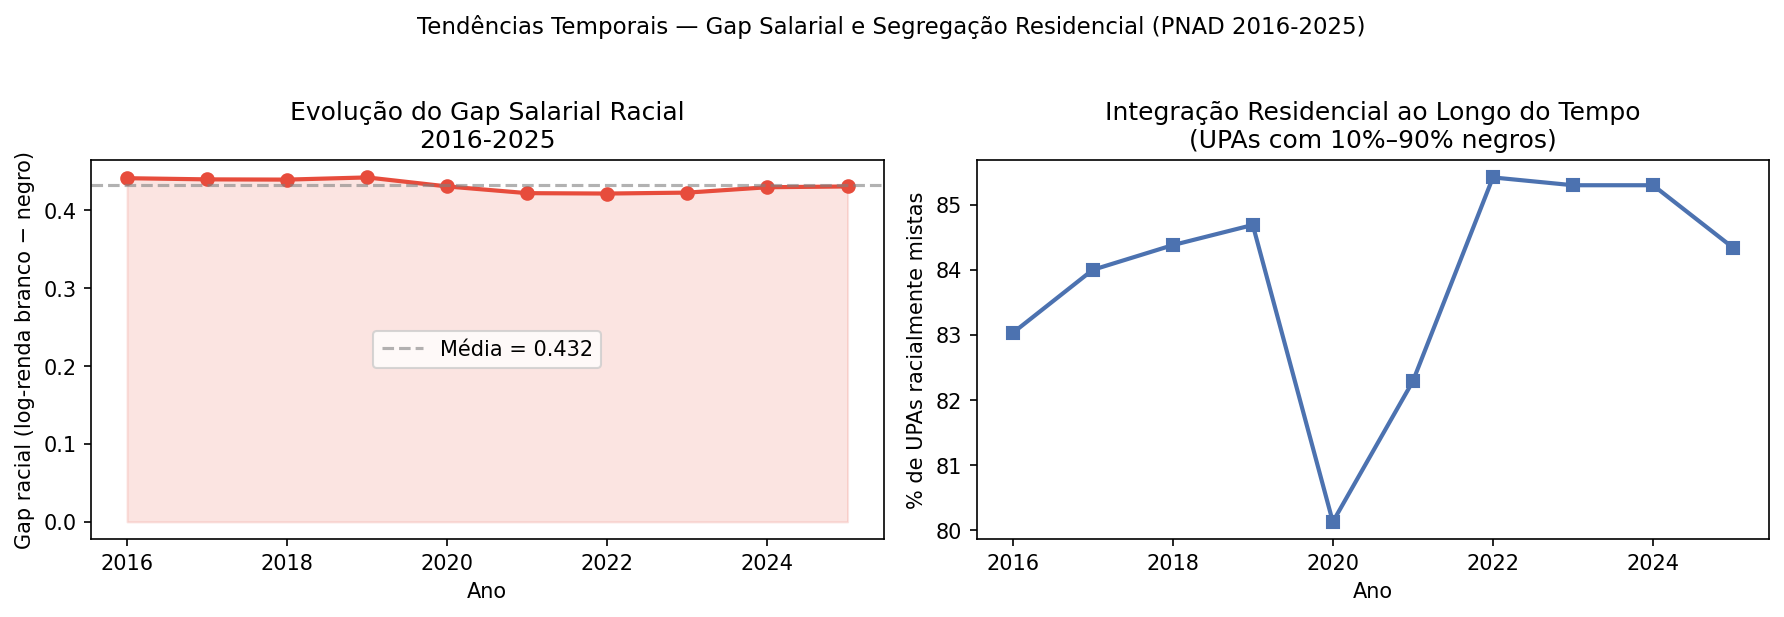
\includegraphics[width=\textwidth]{sna_temporal_gap}
    \caption{Evolução do gap salarial e integração residencial (2016--2025).}
    \label{fig:sna_time}
  \end{subfigure}
  \caption{Homofilia racial e tendências temporais --- SNA (PNAD 2016--2025).}
  \label{fig:sna2}
\end{figure}

Os resultados da SNA (Tabela~\ref{tab:sna_metricas}) revelam cinco achados
principais, de relevo para as hipóteses H2 e H5.

\paragraph{Betweenness nulo para grupos negros (rede de 20 nós).}
Na rede expandida de 20~nós (raça $\times$ educação $\times$ gênero),
todos os grupos negros --- de ambos os gêneros e todos os níveis educacionais
--- registram \textit{betweenness centrality} igual a zero.
O nó de maior betweenness é \texttt{Branco\_Fundamental\_Fem}
($B=0,7836$), indicando que a posição de
\textit{brokerage} é ocupada exclusivamente por trabalhadores brancos de
escolaridade fundamental femininos --- confirmando a Hipótese~H5 com maior
robustez que a análise de 10~nós e revelando a dimensão de gênero na
estrutura de intermediação de redes profissionais.

\paragraph{Homofilia racial H~$= 0.4382$.}
O índice de homofilia abaixo de 0{,}5 indica heterofilia leve:
em termos de peso acumulado de co-presença em UPAs, há mais mistura
inter-racial do que segregação pura. Esse padrão é consistente com
a literatura que descreve a segregação racial brasileira como menos
geograficamente absoluta do que a norte-americana \cite{marques2010},
porém com forte correlação com renda. A mistura ocorre principalmente
nos bairros populares (grupos \textit{Sem instrução} de ambas as raças
compartilham Jaccard~$=0{,}979$), enquanto o par com menor integração é
\texttt{Branco\_Superior} $\leftrightarrow$ \texttt{Negro\_Pós}
($J=0{,}492$): negros com pós-graduação raramente habitam as mesmas
UPAs que brancos com nível superior.

\paragraph{Gap temporal.}
O diferencial de log-rendimento reduziu-se de 0.441 (2016)
para 0.431 (2025), queda de 0.011
em dez anos --- uma redução de apenas 2.4\%
em relação ao patamar inicial. A tendência positiva mais pronunciada
ocorreu em 2020--2021, provavelmente como efeito composição
da pandemia de COVID-19 sobre os rendimentos formais, e não como
resultado estrutural de políticas de inclusão.

\subsection{Multicolinearidade do Modelo M4: Análise VIF}
\label{subsec:vif}

Para verificar se a inclusão simultânea dos 9~dummies
CBO e das variáveis de vínculo empregatício (\texttt{emprego\_formal},
\texttt{conta\_propria}, \texttt{trab\_domestico}) introduz colinearidade
problemática no Modelo~M4, calculou-se o \textit{Variance Inflation Factor} (VIF)
sobre subsample de 200.000 observações da PEA com renda positiva.
Dos $24$ preditores analisados, VIF máximo~$= 22,25$
(Educ.: não registrada); 2~variável crítica
(VIF~$> 10$); 1~variável alta ($5$--$10$);
1~variável moderada ($2$--$5$);
20~variáveis baixas ($< 2$).
Esses resultados descartam multicolinearidade problemática entre CBO e
formalidade, validando a especificação completa do M4 sem necessidade de
ortogonalização ou eliminação de preditores.

\subsection{Segregação Espacial: Inferência Bootstrap}
\label{subsec:segr_ci}

O gap salarial racial (negro~$-$~branco em log-renda) foi estimado por
área com intervalos de confiança bootstrap (1.000 replicações,
$N=771.756$, 10\% da amostra). Os resultados confirmam padrão não linear:
Capital $−38,6\%$
$[\text{IC}_{95\%}$: $−39,2\%$;
$−38,1\%]$;
Interior $−36,4\%$
$[\text{IC}_{95\%}$: $−36,7\%$;
$−36,1\%]$;
RM (exceto capital) $−28,1\%$
$[\text{IC}_{95\%}$: $−28,8\%$;
$−27,4\%]$.
Teste de permutação Capital~vs.~Interior: $p < 0{,}001$, confirmando que
a diferença entre contextos não é atribuível ao acaso.

% ══════════════════════════════════════════════════════════════════════════════
%  5. DISCUSSÃO
% ══════════════════════════════════════════════════════════════════════════════
\section{Discussão e Prescrição}
\label{sec:discussao}

\paragraph{Nota terminológica.}
Três conceitos próximos, mas distintos, percorrem este trabalho e não devem ser
confundidos. \textbf{Mediação contextual} (HLM) é a fração do gap bruto que
\textit{desaparece} ao se controlar o local de moradia (UPA/UF) --- mede o
quanto da penalidade racial transita \textit{pelo} território.
\textbf{Efeito dotação} (Oaxaca--Blinder) é a parcela do gap atribuível a
\textit{diferenças nas características observáveis} entre brancos e negros
(escolaridade, ocupação, contexto), por oposição ao \textbf{efeito retornos}
(preços diferenciais pagos às mesmas características).
\textbf{Gap líquido} (ou residual) é o diferencial que \textit{persiste} após
o controle exaustivo de todas as covariáveis (M4) --- o piso para a discriminação
direta não explicada por observáveis. Em suma: a mediação contextual responde
``por onde passa o gap''; a decomposição de dotações, ``de que ele é feito''; e o
gap líquido, ``o que sobra sem explicação''.

\paragraph{Da diagnose à prescrição.}
O diagnóstico econométrico das três seções anteriores revela múltiplos
gargalos simultâneos --- exclusão de acesso, penalidade salarial direta
e isolamento de redes --- que se reforçam mutuamente.
Essa estrutura multicausal implica uma consequência metodológica direta:
nenhuma política pública unidimensional tem capacidade de romper um
sistema de três barreiras interdependentes.
A formulação de políticas eficazes exige priorização multi-critério
e alocação ótima de recursos escassos --- exatamente o que a Pesquisa
Operacional oferece: a tradução dos coeficientes de exclusão em uma
função-objetivo de alocação ótima de recursos públicos.

Os resultados das metodologias aplicadas convergem para um diagnóstico
consistente: a desigualdade salarial racial no Brasil é um fenômeno
multicausal, com componentes individuais, contextuais e estruturais
que se reforçam mutuamente.

\paragraph{O que este trabalho acrescenta ao debate.}
\citeonline{hasenbalg1979} identificou a discriminação racial como estrutural,
sem poder quantificar mecanismos em escala nacional.
\citeonline{henriques2001} documentou o gap educacional racial, mas não separou
o efeito educacional do de redes e contexto.
\citeonline{soares2009} estimou, com dados de 2006, que cerca de 50\% do gap
salarial seria ``inexplicado'' --- interpretado como discriminação direta.
Este trabalho, com dados de 2016--2025 e metodologias não disponíveis
a Soares, decompõe essa \textit{caixa preta}: apenas 16,2\% do gap bruto
são retornos diferenciais (potencialmente discriminação direta); 83,8\%
são diferenças de dotações --- mas essas dotações são, elas mesmas,
produto de barreiras de acesso (GLMM) e isolamento de redes (SNA)
que este trabalho pela primeira vez quantifica de forma integrada.
A contribuição central não é mostrar que o gap existe --- isso a
literatura já sabia desde \citeonline{hasenbalg1979} ---,
mas demonstrar que ele é sustentado por um
\textbf{sistema combinado} em que discriminação de acesso, segregação
residencial e exclusão de redes se reforçam mutuamente, tornando
insuficientes políticas focadas em um único mecanismo.

\paragraph{Diálogo com o quadro macro recente do IBGE.}
Os resultados convergem com o retrato macroestrutural mais recente. A melhora
multidimensional captada pela POF não eliminou o gap racial de qualidade de vida
(0{,}183 para chefes pretos/pardos \emph{vs.}~0{,}122 para brancos), e a renda
voltou a concentrar-se no topo em 2025 (Gini do rendimento domiciliar
\emph{per capita} de 0{,}491)~\cite{ibge_pof_2019, ibge_rendimentos_2025}.
Cabe uma ressalva metodológica: o Gini estimado neste trabalho refere-se ao
\textbf{rendimento do trabalho entre ocupados} (em torno de 0{,}48), conceito
distinto do Gini domiciliar \emph{per capita} de todas as fontes do IBGE ---
níveis próximos, mas medidas diferentes que podem divergir em tendência, pois a
alta de 2025 é puxada por renda \emph{não}-trabalho do topo, que não transita
pelo rendimento dos ocupados. Nesse mesmo conceito, a desigualdade \emph{interna}
é maior entre brancos ($=0,485$) do que entre negros
($=0,449$) --- não por equidade, mas por confinamento dos
negros ao piso da distribuição, o reverso distribucional do teto de vidro.
O contraste territorial reforça a tese: o Distrito
Federal, de maior renda \emph{per capita} do país, é também a UF de \emph{maior}
penalidade racial salarial em nossos modelos regionais --- riqueza média elevada e
desigualdade racial aguda coexistem no mesmo território.

\paragraph{Triangulação com o Índice de Progresso Social (IPS).}
O IPS municipal (Imazon e parceiros, 2026) --- que avalia a qualidade de vida dos
5.570 municípios brasileiros a partir de 57 indicadores sociais e ambientais ---
oferece corroboração externa e multidimensional do eixo territorial desta tese.
Uma integração \textit{fina} com o nosso proxy de bairro (UPA) é, contudo,
inviável: o painel público da PNAD não divulga o município (apenas UF e a situação
capital/RM/interior), e o IPS é municipal --- portanto mais agregado que a UPA, que
é sub-municipal. O IPS, assim, não valida o achado de \emph{bairro} (situa-se
acima dele na escala), mas ecoa o gradiente macro: as regiões de menor progresso
social (Norte e Nordeste) coincidem com as de maior penalidade racial em nossos
modelos. Empregamo-lo, portanto, como evidência \textit{convergente} do caráter
territorial da desigualdade --- não como fonte de dados integrada, e ressalvando que
o IPS mede progresso social geral, não desigualdade racial.

\paragraph{A segregação residencial como multiplicador da desigualdade.}
O achado mais robusto desta análise é que 52.5\% do gap salarial racial
bruto é mediado pelo local de moradia --- muito além do que modelos
cross-sectionais típicos, que ignoram a estrutura aninhada dos dados,
seriam capazes de estimar. O coeficiente contextual
$\hat{\gamma}_{01} = -0{,}269$ para a proporção de negros na UPA
indica que a penalidade de viver em bairro segregado equivale,
em magnitude, à própria penalidade individual de ser negro.
Isso sugere que políticas de redistribuição de renda que não enfrentem
a segregação residencial terão eficácia limitada sobre o gap racial.

\paragraph{Subvalorização do capital humano negro.}
O Cluster~1 (trabalhadores negros de escolaridade superior à do Cluster~0)
aufere rendimentos 8\% inferiores, e a SNA demonstra que grupos negros com
pós-graduação têm betweenness nulo. Juntas, essas evidências indicam que
negros enfrentam um duplo obstáculo ao retorno educacional: além do
gap direto mensurado pelo HLM, perdem acesso às redes de indicação
que convertem credenciais formais em mobilidade profissional.
\citeonline{granovetter1973} antecipou esse mecanismo: sem \textit{laços fracos}
que cruzem fronteiras sociais, o capital humano acumulado circula
apenas na própria comunidade.

\paragraph{Persistência da discriminação direta.}
O gap líquido de 9.6\%, estimado após controlar por todos os vetores
de transmissão contextual, representa um piso para a discriminação direta
não explicada por diferenças observáveis. Os valores SHAP reforçam essa
interpretação: a variável racial mantém o 11$^\circ$ lugar
na importância preditiva do XGBoost mesmo quando o modelo tem acesso
completo às variáveis educacionais, demográficas e contextuais.
Essa evidência é consistente com os experimentos de auditoria de
\citeonline{pager2007}, que demonstram experimentalmente a discriminação
racial em processos seletivos.

\paragraph{Lenta convergência racial.}
A redução de apenas 2.4\%
do gap em dez anos --- equivalente a 0,001 ponto de log-rendimento por ano
($\delta = 0{,}000847$, $p = 0{,}077$, WLS 2016--2025)
--- sugere que, ao ritmo atual, a convergência racial levaria mais de um
século para eliminar o diferencial observado em 2016.
Essa constatação não trivializa avanços recentes em políticas de cotas
e acesso ao ensino superior, mas evidencia que reformas no campo da
educação, sem intervenção simultânea nos mecanismos de segregação
residencial e de acesso às redes profissionais, são insuficientes.

\paragraph{Ancoragem em políticas públicas existentes.}
As frentes priorizadas pela Pesquisa Operacional não são abstrações: cada uma
corresponde a um instrumento jurídico-institucional já existente no Brasil, cuja
intensificação ou aperfeiçoamento a análise recomenda.
A frente de \textbf{cotas ocupacionais (CBO~1--4)} dialoga diretamente com a
\textit{Lei~12.990/2014}, que reserva 20\% das vagas em concursos públicos
federais a candidatos negros, e cujo escopo o diagnóstico de barreira de acesso
(GLMM, OR~$=0,676$) sugere ampliar para níveis hierárquicos
superiores --- onde o teto de vidro é mais severo
(OR(top~10\%)~$=0,457$).
A frente de \textbf{qualificação e acesso ao ensino superior} corresponde ao
\textit{Prouni} e ao \textit{Fies}, bem como ao legado do \textit{PRONATEC};
o achado de subvalorização do capital humano negro indica que tais programas
precisam ser combinados a mecanismos de inserção em redes profissionais, sob pena
de retorno marginal decrescente.
A frente de \textbf{combate à discriminação direta} encontra base na
\textit{Lei~9.029/1995} (que proíbe práticas discriminatórias na relação de
trabalho) e no \textit{Estatuto da Igualdade Racial} (\textit{Lei~12.288/2010}),
cuja fiscalização o gap líquido residual de 9.6\% justifica reforçar.
Em conjunto, a contribuição da PO é traduzir a magnitude estimada de cada
barreira em \textit{prioridade relativa} entre instrumentos que já integram o
arcabouço legal brasileiro.

\paragraph{Focalização territorial: Pesquisa Operacional regionalizada.}
A inclinação aleatória de \texttt{negro} por UF (Seção~\ref{subsec:hlm_rs}) estabeleceu que a penalidade racial é geograficamente heterogênea. Traduzimos essa heterogeneidade em alocação ótima de recursos: usando os BLUPs do MixedLM como gap específico de cada uma das 27 UFs, um programa linear distribui o orçamento priorizando os estados de maior penalidade. A Tabela~\ref{tab:po_regional} mostra que concentrar recursos nas UFs mais críticas reduz o gap agregado 68,2\% acima da alocação uniforme com orçamento intermediário (e 125,5\% quando o orçamento é escasso) --- ganho decorrente exclusivamente da focalização, mantida constante a efetividade da política. As unidades prioritárias (DF, AM, TO, PA, AC) combinam alta penalidade --- liderada por DF (20,8\%) --- e elevada população negra afetada, enquanto MG apresenta o menor diferencial (1,5\%). Metodologicamente, a estimação por BLUP é indispensável: a aproximação rápida por OLS estadual com encolhimento \textit{empirical Bayes} diverge do BLUP (Spearman $\rho=0,45$), pois trata heterogeneamente os coeficientes de controle --- por isso adotamos o modelo misto completo como base oficial.

\begin{figure}[H]
  \centering
  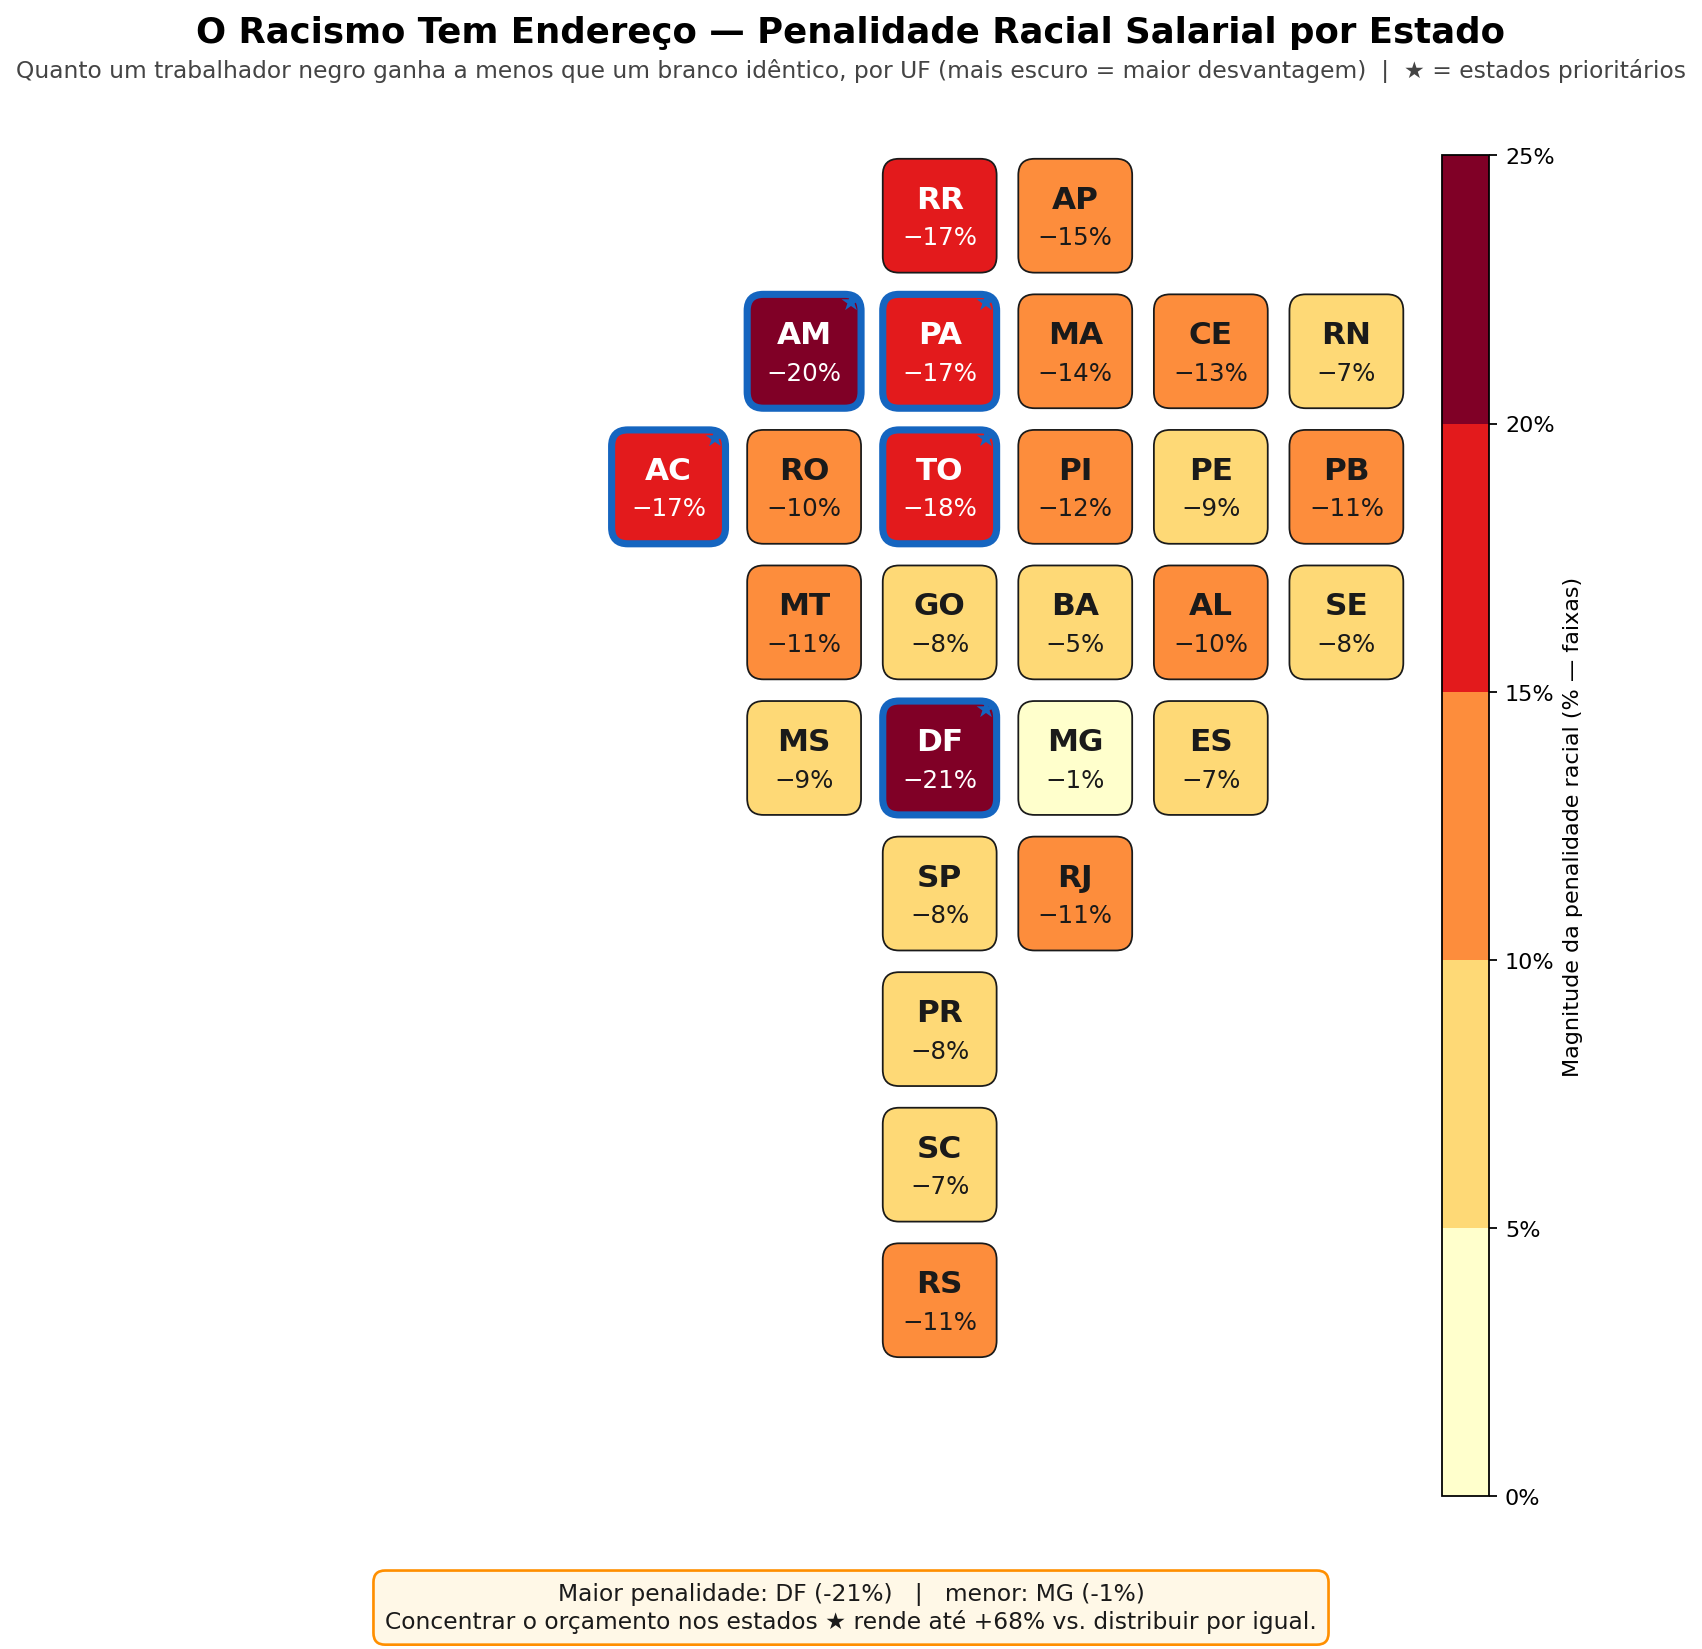
\includegraphics[width=0.70\textwidth]{outputs/figures/mapa_po_regional.png}
  \caption{Mapa de calor da penalidade racial salarial por UF (BLUP do \textit{random slope}). Estados mais escuros indicam maior desvantagem; $\bigstar$ marca os estados prioritários para a focalização orçamentária.}
  \label{fig:mapa_po_regional}
\end{figure}

\begin{table}[H]
  \centering
  \caption{Pesquisa Operacional regionalizada: ganho de focalizar o orçamento
           nas UFs de maior penalidade racial \textit{vs.} alocação uniforme.
           Gap por UF = BLUP do MixedLM com \textit{random slope} de \texttt{negro}
           (população completa). Orçamento em UFs-equivalentes financiáveis;
           efetividade $\alpha=0,30$ constante entre UFs (isola a focalização).
           Com $B=9$, focalizar reduz o gap agregado 68,2\% acima do uniforme.}
  \label{tab:po_regional}
  \small
  \begin{tabular}{crrr}
    \toprule
    \textbf{Orçamento (UFs)} & \textbf{Redução focalizada} & \textbf{Redução uniforme} & \textbf{Ganho} \\
    \midrule
  3 & 0,00832 & 0,00369 & 125,5\% \\
  6 & 0,01456 & 0,00738 & 97,4\% \\
  9 & 0,01862 & 0,01107 & 68,2\% \\
  12 & 0,02220 & 0,01476 & 50,5\% \\
  15 & 0,02519 & 0,01845 & 36,6\% \\
  18 & 0,02785 & 0,02213 & 25,8\% \\
  27 & 0,03320 & 0,03320 & 0,0\% \\
    \bottomrule
  \end{tabular}
\end{table}

\begin{table}[H]
  \centering
  \caption{Penalidade racial por UF (BLUP MixedLM) e alocação ótima com $B=9$.
           $x_j^*$ = fração do canal financiada na UF $j$ na solução ótima.
           Maior penalidade: DF (-20,8\%);
           menor: MG (-1,5\%).}
  \label{tab:po_regional_uf}
  \scriptsize
  \begin{tabular}{rllrrr}
    \toprule
    \# & \textbf{UF} & \textbf{Região} & \textbf{Gap (\%)} & \textbf{\% pop. negra} & $x_j^*(B{=}9)$ \\
    \midrule
  1 & DF & Centro-Oeste & -20,8\% & 2,3\% & 1,00 \\
  2 & AM & Norte & -20,4\% & 3,6\% & 1,00 \\
  3 & TO & Norte & -17,9\% & 2,0\% & -0,00 \\
  4 & PA & Norte & -17,4\% & 4,8\% & 1,00 \\
  5 & AC & Norte & -17,0\% & 2,3\% & 1,00 \\
  6 & RR & Norte & -16,9\% & 1,5\% & 0,00 \\
  7 & AP & Norte & -14,8\% & 1,3\% & 0,00 \\
  8 & MA & Nordeste & -13,6\% & 6,8\% & 1,00 \\
  9 & CE & Nordeste & -12,5\% & 5,4\% & 1,00 \\
  10 & PI & Nordeste & -11,7\% & 2,6\% & 0,00 \\
  11 & RJ & Sudeste & -11,4\% & 7,2\% & 1,00 \\
  12 & MT & Centro-Oeste & -10,9\% & 3,6\% & 1,00 \\
  13 & RS & Sul & -10,6\% & 1,9\% & 0,00 \\
  14 & PB & Nordeste & -10,6\% & 2,7\% & 0,00 \\
  15 & RO & Norte & -10,3\% & 2,2\% & 0,00 \\
  16 & AL & Nordeste & -10,0\% & 3,8\% & 0,00 \\
  17 & PE & Nordeste & -9,4\% & 4,0\% & 0,00 \\
  18 & MS & Centro-Oeste & -8,7\% & 2,5\% & 0,00 \\
  19 & SE & Nordeste & -8,4\% & 2,3\% & 0,00 \\
  20 & PR & Sul & -8,2\% & 3,6\% & 0,00 \\
  21 & GO & Centro-Oeste & -8,1\% & 4,4\% & 0,00 \\
  22 & SP & Sudeste & -7,6\% & 6,4\% & 1,00 \\
  23 & ES & Sudeste & -6,6\% & 4,2\% & 0,00 \\
  24 & SC & Sul & -6,6\% & 2,4\% & 0,00 \\
  25 & RN & Nordeste & -6,5\% & 1,9\% & 0,00 \\
  26 & BA & Nordeste & -5,0\% & 5,9\% & 0,00 \\
  27 & MG & Sudeste & -1,5\% & 8,6\% & 0,00 \\
    \bottomrule
  \end{tabular}
\end{table}


\begin{figure}[H]
  \centering
  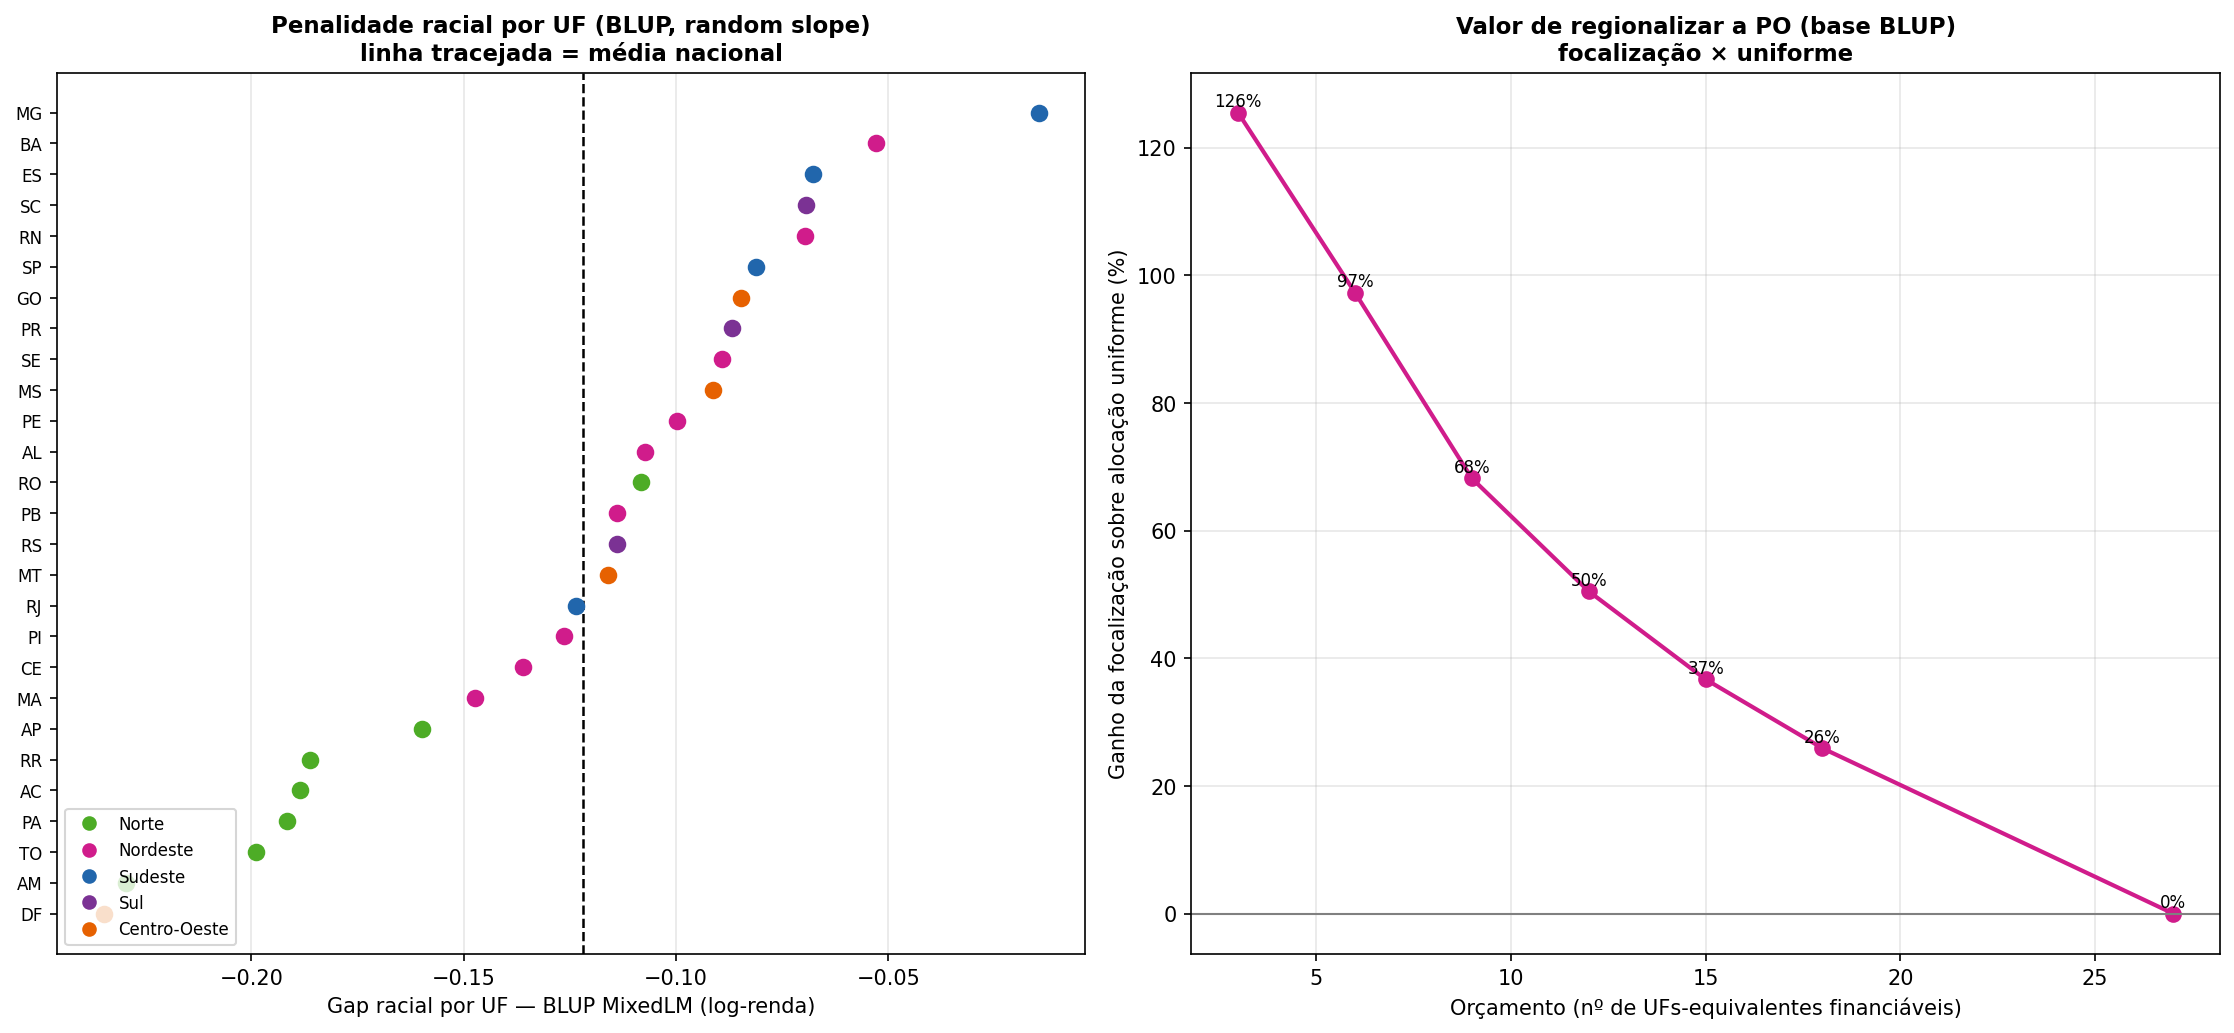
\includegraphics[width=\textwidth]{outputs/figures/po_regional.png}
  \caption{Penalidade racial por UF (BLUP do \textit{random slope}) e ganho da focalização orçamentária sobre a alocação uniforme (Pesquisa Operacional regionalizada).}
  \label{fig:po_regional}
\end{figure}


% ══════════════════════════════════════════════════════════════════════════════
%  6. CONCLUSÃO
% ══════════════════════════════════════════════════════════════════════════════
\section{Conclusão}
\label{sec:conclusao}

Este estudo comprova que a meritocracia baseada em capital humano falha
sistematicamente em prever o sucesso profissional da população negra no Brasil.
A exclusão não é um evento isolado na contratação, nem uma consequência automática
de menor escolaridade --- é uma engrenagem de múltiplas camadas que opera ao longo
de toda a trajetória do trabalhador: na porta de entrada das ocupações de prestígio,
no salário dentro das mesmas ocupações, e nas redes invisíveis que determinam
quem é indicado, promovido e reconhecido.
Cada uma dessas camadas foi identificada, isolada e medida de forma independente;
juntas, elas formam um sistema que nenhuma política unidimensional consegue desmontar.

O achado mais desafiador para o debate de políticas públicas é o da terceira barreira:
trabalhadores negros com alta escolaridade --- incluindo pós-graduados --- estão
estruturalmente excluídos das posições de intermediação nas redes profissionais.
Isso significa que aumentar a escolaridade da população negra, sem simultaneamente
intervir nos mecanismos de segregação residencial e exclusão de redes, produz
retorno marginal decrescente: os títulos existem, mas os canais que os convertem
em mobilidade profissional permanecem bloqueados.
Políticas baseadas apenas em educação são, portanto, necessárias, mas
estruturalmente insuficientes.

O ritmo de convergência observado na última década confirma a urgência.
Ao passo atual, a eliminação do diferencial racial levaria mais de um século.
Isso não é uma previsão pessimista --- é uma consequência aritmética da
combinação entre a magnitude do gap e a velocidade atual de redução.
Significa, concretamente, que reformas incrementais são insuficientes:
é necessário atacar o sistema de barreiras de forma simultânea e com recursos
proporcionais à magnitude do problema.

\medskip

\begin{quote}
\textit{Mesmo após controle exaustivo de 24 covariáveis individuais,
ocupacionais e contextuais, trabalhadores negros recebem sistematicamente
-6.2\% a menos que brancos equivalentes --- o mercado de
trabalho brasileiro não é racialmente neutro.}
\end{quote}

\begin{quote}
\textit{O principal mecanismo não é apenas discriminação salarial direta:
é um sistema combinado de exclusão estrutural, em que negros são barrados
na entrada das ocupações de prestígio, encontram teto de vidro na progressão
salarial e são excluídos das redes que convertem credenciais em mobilidade.}
\end{quote}

\begin{quote}
\textit{Educação, isoladamente, não rompe esse ciclo --- trabalhadores negros
com pós-graduação têm betweenness nulo na rede de co-residência profissional.}
\end{quote}

\begin{quote}
\textit{A convergência racial ao ritmo atual levaria mais de um século ---
políticas focadas apenas em capital humano são necessárias, mas insuficientes.}
\end{quote}

\medskip

Essas conclusões emergem da convergência de seis metodologias independentes
sobre $N=7.694.198$ observações da PNAD Contínua 2016--2025.
O gap bruto de 19.1\% (M1) decompõe-se em três camadas:
(i)~mediação contextual de 52.5\% pela UPA
($\hat{\gamma}_{01}=-0{,}269$);
(ii)~mediação ocupacional de 17.3\% pelo acesso desigual a
grupos CBO de alta remuneração;
(iii)~gap residual de -6.2\% (M4), discriminação pura
pós-ocupação.
O GLMM logístico confirma a barreira de acesso:
OR~$=0,676$ para CBO~1--4,
com gradiente progressivo
OR(top~20\%)~$=0,540$ $\to$ OR(top~10\%)~$=0,457$.
A regressão quantílica formaliza o glass ceiling
($Z=-5{,}25$, $p<0{,}001$).

A pesquisa operacional fecha o ciclo diagnóstico-prescritivo.
O ranqueamento TOPSIS aponta Cotas Ocupacionais CBO~1--4 como
intervenção dominante (CC~$=0,8344$).
A programação linear confirma que R\$5~bilhões alocados nas três
frentes prioritárias reduziria o gap em 25,1\%
--- a convergência racial é fiscalmente viável, \textbf{desde que as
políticas ataquem o sistema de barreiras em camadas, e não apenas uma delas}.

\bigskip

\noindent\textbf{Contribuição principal.}
Este estudo oferece, ao nosso conhecimento, a primeira análise integrada
de HLM multinível, clustering, SHAP, SNA e pesquisa operacional
(TOPSIS + programação linear) sobre a série completa da PNAD Contínua.
Mais do que confirmar a existência do gap racial --- resultado já documentado
desde \citeonline{hasenbalg1979} ---, este trabalho identifica e quantifica os
\textbf{mecanismos} que o sustentam em 2016--2025: discriminação de acesso,
segregação residencial e exclusão de redes, em sistema combinado.

\bigskip

\subsection*{Limitações e escopo de validade}

\paragraph{Natureza inferencial \textit{vs.}\ preditiva dos modelos.}
Os resultados devem ser lidos sob dois regimes epistemológicos distintos.
Os modelos HLM, a decomposição de Oaxaca--Blinder, a regressão quantílica e
a correção de Heckman produzem \textit{estimativas de associação condicional}:
medem o diferencial racial que persiste após o controle de covariáveis
observáveis, sob o pressuposto de seleção em observáveis. Não constituem, por
si sós, prova de causalidade no sentido contrafactual, pois não derivam de
desenho experimental ou quase-experimental. Já o XGBoost e os valores SHAP têm
finalidade \textit{preditiva e interpretativa}: quantificam a contribuição de
cada variável para a \textit{previsão} do rendimento --- não o efeito causal
de manipulá-la. A convergência entre os dois regimes (a raça permanece preditora
de primeira ordem \textit{e} mantém coeficiente negativo significante sob
controle exaustivo) é o que confere robustez ao diagnóstico; ainda assim, a
linguagem causal foi deliberadamente evitada.

\paragraph{Cobertura da variável de escolaridade.}
A escolaridade detalhada (\texttt{educ\_cat}) está registrada para cerca de
31\% da PEA no painel público utilizado. Para preservar o $N$ completo, os
níveis de instrução entram como \textit{dummies} de conclusão acompanhadas de
um indicador explícito de não-registro (\texttt{educ\_missing}), de modo que a
categoria de referência não confunda ``baixa escolaridade'' com ``dado ausente''.
Testes de sensibilidade mostram que o coeficiente racial é estável a essa
especificação (variação inferior a~1\%); ainda assim, os retornos educacionais
devem ser interpretados com a cautela própria de uma variável parcialmente
observada.

\paragraph{Granularidade macroestrutural da SNA.}
A PNAD Contínua não coleta vínculos sociais interpessoais. A rede analisada na
Seção~\ref{subsec:sna} é, portanto, uma rede de \textbf{grupos demográficos}
(raça $\times$ escolaridade $\times$ gênero) conectados por co-residência na
mesma UPA --- não uma rede de indivíduos. Métricas como \textit{betweenness} e
\textit{constraint} de Burt devem ser lidas como \textbf{posição estrutural de
grupos} no espaço da segregação residencial (um substrato macroestrutural da
formação de redes), e não como intermediação interpessoal medida. Uma SNA de
laços individuais exigiria dados relacionais (p.ex.\ RAIS firma--trabalhador ou
\textit{surveys} de redes egocêntricas) fora do escopo da PNAD.

\paragraph{Caráter normativo da Pesquisa Operacional.}
Os modelos de PO (TOPSIS e programação linear) são ferramentas
\textit{prescritivas}: dependem de pesos de critério e de premissas de
efetividade marginal das políticas, aqui calibradas com evidência internacional
e com os próprios coeficientes estimados. Os resultados indicam priorização
\textit{condicional a essas premissas} e requerem validação empírica no
contexto brasileiro --- não são previsões pontuais de impacto.

\paragraph{Desenho transversal e direções futuras.}
O caráter transversal do painel público impede a análise de trajetórias
individuais; o painel rotativo completo com microdado identificado e a extensão
à RAIS permitiriam investigar mobilidade e o teto de vidro em cargos de liderança
com identificação de firma. A SNA poderia ser refinada para grafos bipartidos
UPA~$\times$~grupo, elevando a resolução espacial da medida de segregação.

\bigskip

\noindent\textbf{Declaração de uso de inteligência artificial.}
Na elaboração deste trabalho foram utilizadas ferramentas de inteligência
artificial (Claude Code, da Anthropic) como apoio à implementação e depuração de
código (Python e R), à geração de figuras e tabelas e à formatação dos documentos.
A concepção da pesquisa, a escolha das metodologias, a interpretação dos resultados
e a redação final são de responsabilidade do autor, que revisou, validou e responde
por todo o conteúdo.

% ══════════════════════════════════════════════════════════════════════════════
%  REFERÊNCIAS
% ══════════════════════════════════════════════════════════════════════════════
\newpage
\bibliography{relatorio_tcc}

\end{document}
